\documentclass[11pt]{article}
\usepackage[margin=1in]{geometry}
\usepackage[T1]{fontenc}
\usepackage[utf8]{inputenc}
\usepackage{lmodern,microtype}
\usepackage{amsmath,amssymb,amsthm,mathtools}
\usepackage{graphicx,booktabs,array,enumitem,setspace,placeins}
\usepackage{algorithm}
\usepackage{algpseudocode}
\usepackage{needspace}
\usepackage[authoryear,round]{natbib}
\usepackage[colorlinks=true,allcolors=blue]{hyperref}
\usepackage{bookmark}
\allowdisplaybreaks
\setstretch{1.18}
\setlength{\parskip}{0pt}
\setlength{\emergencystretch}{2em}
\setlist{itemsep=2pt,topsep=4pt}
\newtheorem{theorem}{Theorem}[section]
\newtheorem{lemma}[theorem]{Lemma}
\newtheorem{proposition}[theorem]{Proposition}
\newtheorem{corollary}[theorem]{Corollary}
\newtheorem{definition}[theorem]{Definition}
\newtheorem{example}[theorem]{Example}
\theoremstyle{remark}
\newtheorem{remark}[theorem]{Remark}
\newcommand{\E}{\mathbb E}
\newcommand{\Prob}{\mathbb P}
\newcommand{\ind}{\mathbf 1}
\newcommand{\kl}{\operatorname{kl}}
\newcommand{\pos}[1]{\left[#1\right]_+}
\newcommand{\suppproof}{Complete proofs appear in the supplementary material.}

\renewcommand{\thesection}{S\arabic{section}}
\renewcommand{\thepage}{S-\arabic{page}}
\title{Supplement to ``Multi-armed bandits with arriving arms:\\sequential screening and reliable set maintenance''}
\author{}
\date{October 15, 2026}
\begin{document}
\maketitle
\section*{Notation and scope}
The observation model has independent arm streams, each consisting of
independent, identically distributed rewards in $[0,1]$, deterministic
permanent arrivals $\mathcal{A}_t$, and one observation per physical time step.
Let $r^*(t)=\max_{i\in \mathcal{A}_t}r_i$, $\Delta_i(t)=r^*(t)-r_i$, and
$\mathcal G_t^\varepsilon=\{i:\Delta_i(t)\le\varepsilon\}$. Reports are issued after
the current observation and partition $\mathcal{A}_t$ as $(\mathcal P_t,\mathcal N_t,\mathcal V_t)$. Write
\[
 E_{\rm lab}=\{\forall t:\mathcal P_t\subseteq \mathcal G_t^\varepsilon
                             \subseteq \mathcal{A}_t\setminus \mathcal N_t\},\qquad
 \mathcal U_T(\eta)=\sum_{t\le T}\sum_{i\in \mathcal{A}_t}
 \ind\{i\in \mathcal V_t,|\Delta_i(t)-\varepsilon|>\eta\},
\]
and $R_T=\sum_{t\le T}\Delta_{I_t}(t)$. Reliability means
$P(E_{\rm lab})\ge1-\delta$ for every allowed environment.
$\mathfrak R_\Theta(a)$ minimizes worst-case $ER_T$ over full-model reliable
policies with $P_\theta(E_{\rm lab},\mathcal U_T\le a)\ge1-\delta$ for all
$\theta\in\Theta$. A bar denotes averaging under the independent uniform
prior on all candidate signs. These priors are proof devices and impose no
Bayesian requirement on the policy.

All probability and sample-budget interfaces are proved below. Classical
change of measure and multiple-recovery scales are credited to the existing
literature \citep{kaufmann2016,malloy2014,jamieson2018,mason2020}.

% Complete proof for the original screening architecture, with explicitly
% repaired comparison, confidence calibration, and physical stopping rules.
% This file does not prove a claim about CP-UCB-AA or inherit the former G3 bound.
\section{A fixed-budget analysis of the screening-based UCB-AA procedure}
\label{app:ucbaa_repaired}

\subsection{Exact scope and executable conventions}

Fix a deterministic physical horizon $T\ge1$ and $0<\delta<1$.
There are finitely many available arms by every finite time, at least one arm
is available at time one, and arrivals are deterministic and permanent.
The arm streams are independent, and each consists of iid $[0,1]$-valued
rewards with mean $r_i$. The proof also applies conditionally on an independent exogenous
arrival schedule. No gap-stability or cumulative-jump assumption is imposed.
The learner observes the arrivals before selecting the arm at each physical
time. Newly arriving arms are buffered until the next algorithmic round.
All observations are retained, and an eliminated arm is not sampled again.

Set
\begin{equation}
 M_T=\left\lceil\frac12\log_2(T+1)\right\rceil,\qquad
 N=\frac{8T4^{M_T}}{\delta},\qquad \widetilde\Delta_p=2^{-p},
 \label{eq:ucbaa_calibration}
\end{equation}
and, for $0\le p\le M_T$, retain the original target and radius formulas
\begin{equation}
 n_p=\left\lceil
       \frac{2\log(N\widetilde\Delta_p^2)}{\widetilde\Delta_p^2}
       \right\rceil,\qquad
 b_p=\sqrt{\frac{\log(N\widetilde\Delta_p^2)}{2n_p}}.
 \label{eq:ucbaa_targets}
\end{equation}
The calibration in \eqref{eq:ucbaa_calibration} is a sufficient choice for
this theorem; the smaller empirical calibration in the submitted version
is not covered by this probability guarantee.

Write $s_m$ for the physical starting time of algorithmic round $m$, with
$s_0=1$. At $s_m$ admit every arm in the buffer, including arrivals at $s_m$.
The admitted batch is $A_m$, its cumulative union is $A(m)$, the incumbent
survivors are $C_{m-1}$, and the initial active set is
$B_m=C_{m-1}\cup A_m$. Put $C_{-1}=\varnothing$.
These are the round-based sets of the original UCB-AA procedure. Its
notation $K(m)$, when used, denotes a prescribed nondecreasing upper
bound on $|A(m)|$; it is different from the actual physical-time count
$K_t=|\mathcal A_t|$. This proof does not require $K(m)$ as an additional
input because the calibration controls at most $T$ observed streams.

The following conventions make the original two-stage architecture precise.
They are part of the analyzed procedure, not conclusions about unspecified
implementations.
\begin{enumerate}
 \item An elimination call at phase $p$ first samples every arm in its
 candidate set $S$ until its lifetime count reaches $n_p$. An arm already
 at or above that target receives no additional sample. After the entire
 call's sampling is complete, form
 \[
  \mathrm{LCB}_i(p)=\hat r_i(n_p)-b_p,\qquad
  \mathrm{UCB}_i(p)=\hat r_i(n_p)+b_p
 \]
 from the actual first $n_p$ observations of each reference arm.
 Remove simultaneously from $S$ exactly those arms for which
 \[
  \mathrm{UCB}_i(p)<\max_{j\in R}\mathrm{LCB}_j(p).
 \]
 In particular, the inequality is strict. Prefix statistics for incumbents
 are retained; an unobserved prefix is never substituted into a comparison.
 \item For $m\ge2$, run preliminary phases $p=0,\ldots,m-2$ on the
 surviving part of $A_m$, with reference set equal to that part together
 with $C_{m-1}$. Only new arms are removed in these calls. Then run formal
 phases $p=m-1,m$ on the merged survivors. For $m=1$, run only formal
 phases $0,1$; for $m=0$, run formal phase $0$.
 \item If a new batch is empty, all its preliminary phases are no-ops:
 the set entering formal phase $m-1$ is $C_{m-1}$. An empty surviving new
 batch is handled the same way. This specifies the missing intermediate
 set in the original pseudocode when preliminary screening is skipped.
 \item Sampling orders and ties are fixed by observed history and
 independent policy randomization. Every physical pull counts toward
 $T$. Stop immediately after pull $T$, even in the middle of an arm's
 target, an elimination call, or a round. No terminal round is appended
 to remove buffered arrivals from the regret ledger.
\end{enumerate}

Thus the alteration preserves buffering, screening against incumbent
evidence, and formal elimination. It repairs the statistical bookkeeping
and stopping convention; it does not replace UCB-AA by a reward-service
mixture or by CP-UCB-AA.

\subsection{Three distinct contributions to regret}

At a physical time $t\le T$, let $m(t)$ be its current algorithmic round.
Define the best initially active mean and the best admitted mean by
\[
 r_{*(m)}=\max_{i\in B_m}r_i,\qquad
 r_{\mathrm{adm}}(m)=\max_{i\in A(m)}r_i.
\]
For an admitted arm in round $m$, distinguish the original roundwise gap
$\Delta_i^{\mathrm{rd}}(m)=r_{*(m)}-r_i$ from the physical-time gap
$\Delta_i(t)=r^*(t)-r_i$, where
$r^*(t)=\max_{i\in\mathcal A_t}r_i$. The superscript marks the
algorithmic-round clock; it does not alter the physical-time gap definition.
The following three truncated quantities have different meanings:
\begin{align}
 R_{\mathrm{round}}(T)
  &=\sum_{t=1}^T\{r_{*(m(t))}-r_{I_t}\},\nonumber\\
 \mathcal H_T
  &=\sum_{t=1}^T\{r_{\mathrm{adm}}(m(t))-r_{*(m(t))}\},\nonumber\\
 D_T
  &=\sum_{t=1}^T\{r^*(t)-r_{\mathrm{adm}}(m(t))\}.
 \label{eq:ucbaa_three_terms}
\end{align}
Here $\mathcal H_T$ is the deficit caused by previously eliminated admitted arms,
whereas $D_T$ is arrival delay alone. On every sample path,
\begin{equation}
 R_T(\pi)=R_{\mathrm{round}}(T)+\mathcal H_T+D_T.
 \label{eq:ucbaa_exact_identity}
\end{equation}
All three terms are nonnegative, since the selected arm belongs to $B_{m(t)}$
and $B_{m(t)}\subseteq A(m(t))\subseteq\mathcal A_t$.
In particular, the residual after subtracting roundwise regret is not in
general arrival delay alone.

For a prescribed complete run of $M+1$ algorithmic rounds, the original
$T_0(\pi)$ denotes its actual, generally random number of pulls, and
$R_{\mathrm{round}}(T_0(\pi))=R_M(\pi)$. The identity
\eqref{eq:ucbaa_exact_identity} applies at that completed endpoint as a
pathwise accounting statement. The fixed-budget theorem below does not
replace a deterministic $T$ by $\mathbb E T_0(\pi)$ or assert an
unproved bound at an arbitrary stopping time.

Arrival delay has an exact exposure representation, including an unfinished
last round. Let $\beta_u=r^*(u)-r^*(u-1)\ge0$ for $u\ge2$, and define
\[
 \alpha_T(u)=\min\bigl(\{s_m:u\le s_m\le T\}\cup\{T+1\}\bigr).
\]
Because every available arm is admitted at a round boundary,
$A(m)=\mathcal A_{s_m}$ and $r_{\mathrm{adm}}(m)=r^*(s_m)$.
Changing the order of two finite sums yields
\begin{equation}
 D_T=\sum_{u=2}^T\beta_u\{\alpha_T(u)-u\}.
 \label{eq:ucbaa_delay_exposure}
\end{equation}
An improvement arriving exactly at a round boundary has zero delay.
An improvement that is still buffered at $T$ is charged through $T$.

\begin{theorem}[UCB-AA at a fixed physical budget]
\label{thm:ucbaa_fixed_budget}
Under the model and executable conventions above, let
$K_T=|\mathcal A_T|$. With probability at least $1-\delta$, the best
admitted mean is always represented in the active set, $\mathcal H_T=0$, and
\begin{equation}
 R_T(\pi)\le
 \min\left\{T,\ 8\sqrt{(2\log N+1)K_TT}+D_T\right\}.
 \label{eq:ucbaa_fixed_hp}
\end{equation}
Consequently
\begin{equation}
 \mathbb E R_T(\pi)\le
 \min\left\{T,\ 8\sqrt{(2\log N+1)K_TT}
                   +\mathbb E D_T+\delta T\right\}.
 \label{eq:ucbaa_fixed_expectation}
\end{equation}
The confidence event and both bounds include the last incomplete round and
all samples in incomplete calls. The statement does not require a unique
best arm and does not compress an elimination-time gap into a terminal gap.
\end{theorem}

\begin{proof}
First check the targets and the stopping convention. Since
$\log(N4^{-M_T})=\log(8T/\delta)>1$, the function
$x\mapsto2x\log(N/x)$ is increasing on $[1,4^{M_T}]$.
More explicitly, its successive phase differences are
\[
 2\,4^{p-1}\{3\log(N4^{-p})-\log4\}>1,\qquad p\ge1.
\]
Therefore $n_p$ is strictly increasing. Also
\begin{equation}
 b_p\le\widetilde\Delta_p/2,\qquad
 n_p\le(2\log N+1)4^p,\qquad n_{M_T}>T.
 \label{eq:ucbaa_target_facts}
\end{equation}
The last fact follows from $4^{M_T}\ge T+1$ and
$\log(N4^{-M_T})>1$. Formal elimination with a strict inequality never
removes every arm, even off the confidence event: an arm with maximal lower
confidence bound cannot satisfy the removal rule because its upper bound
is at least its own lower bound. Initial and subsequent active sets are
therefore nonempty. Completing round $M_T$ would require a surviving arm
to have $n_{M_T}>T$ observations, and hence cannot happen before the
physical stopping time. The finite phase range suffices on every path.

For the global event, order arms by their first observed reward. At most
$T$ streams are exposed by time $T$. An arm's unobserved reward stream is
independent of the history that first selects it, and the bounded iid
Hoeffding inequality is uniform over its mean. For each exposed stream,
the union of its potential-prefix failures over $p=0,\ldots,M_T$ has
probability at most
\[
 \sum_{p=0}^{M_T}2\exp(-2n_pb_p^2)
  =\frac2N\sum_{p=0}^{M_T}4^p
  <\frac{8\,4^{M_T}}{3N}.
\]
Here the potential prefix is defined even if the policy never observes
that many rewards. Applying the same bound conditionally at the first
exposure and summing over at most $T$ exposed streams gives an event $E$
with
\begin{equation}
 \mathbb P(E^c)\le\frac{8T4^{M_T}}{3N}=\frac\delta3\le\delta,
 \qquad
 |\hat r_i(n_p)-r_i|\le b_p
 \label{eq:ucbaa_global_coverage}
\end{equation}
for every observed arm and every phase needed in a comparison.
One direct proof of the concentration inequality used here is as follows.
For a random variable $Z\in[0,1]$, the second derivative of its centered
log moment generating function is a tilted variance and is at most $1/4$.
Twice integrating gives
$\mathbb E e^{\lambda(Z-\mathbb EZ)}\le e^{\lambda^2/8}$.
Multiplication over independent observations and exponential Markov
inequality give the two-sided bound $2e^{-2nx^2}$.
The exposure argument uses only independence of an unrevealed stream,
not independence of its eventual sample count or admission round.
More formally, let $F_i$ be the union of potential-prefix failures for
stream $i$, and let $q=(2/N)\sum_{p=0}^{M_T}4^p$. Before revealing the
reward at time $t$, condition on the observed history and the policy's
current independent randomization. On the event that $I_t$ has never
been sampled, its stream is still unrevealed and the conditional
probability of $F_{I_t}$ is at most $q$. Summing over $t\le T$ bounds
the probability that any first-exposed stream fails by $Tq$.
This conditioning occurs before that stream's first reward is revealed.

Work on $E$. At every comparison, all reference means lie between their
actual lower and upper confidence bounds. A maximal-mean arm in the
reference set cannot satisfy the strict removal inequality. For formal
elimination this preserves the maximum of the entire active set. In
pre-elimination an incumbent maximum is not eligible for removal, and a
new maximum cannot satisfy the removal inequality either. Induction over
calls and rounds shows
\[
 \max_{i\in C_m}r_i=\max_{i\in A(m)}r_i
\]
at every completed round, and the best admitted mean is preserved during
every incomplete round as well. Thus
$r_{*(m)}=r_{\mathrm{adm}}(m)$ and $\mathcal H_T=0$.

There is no unavailable-prefix comparison in this induction. At the end
of round $m-1$, every incumbent survivor has exactly $n_{m-1}$ lifetime
observations. In preliminary phase $p\le m-2$, this includes the stored
first $n_p$ observations. New reference arms have just been sampled to
$n_p$ before the simultaneous comparison. Formal calls likewise have
the requisite prefixes after their sampling step.

Next establish the actual-count invariant. After any completed phase $p$
in round $m$, every eligible arm that survives the comparison has
\begin{equation}
 r_{*(m)}-r_i\le4b_p.
 \label{eq:ucbaa_survival_gap}
\end{equation}
Indeed a maximal-mean reference arm $j$ is still present, so
$\mathrm{LCB}_j(p)\ge r_{*(m)}-2b_p$, whereas
$\mathrm{UCB}_i(p)\le r_i+2b_p$. Survival requires the latter quantity
to be at least the former. This proves
\eqref{eq:ucbaa_survival_gap} without conditioning on a selected estimate.
The claim concerns eligible new arms in a preliminary call and all
survivors in a formal call; no such bound is asserted for untested
incumbents during preliminary screening.

Consider a physical pull that is the $n$th lifetime observation of its arm
and occurs while filling target $n_p$ in round $m$. If $p=0$, its roundwise
gap is at most one. If $p\ge1$ and the arm is new in the current round,
it survived phase $p-1$ of this same round before this pull, and its gap
is at most $4b_{p-1}$. If it is an incumbent, no sample is needed in
formal phase $m-1$, since it already has $n_{m-1}$ observations.
Its new samples occur only in phase $m$, after it survived the current
round's formal phase $m-1$, giving the same bound. This includes $m=1$;
in round zero the only target is $n_0$.
Consequently \eqref{eq:ucbaa_target_facts} gives, for every actual pull,
\begin{equation}
 r_{*(m)}-r_i\le
 \min\left\{1,\ 4\sqrt{\frac{2\log N+1}{n}}\right\}.
 \label{eq:ucbaa_actual_prefix_charge}
\end{equation}
For $p\ge1$, use $4b_{p-1}\le4\widetilde\Delta_p$ and
$n\le n_p\le(2\log N+1)4^p$. For $p=0$, use
$n\le n_0\le2\log N+1$. A partially sampled final phase requires
only the preceding comparison, which has already finished, so the
argument does not presume completion of the final target.

No arm's lifetime count is reset. Summing the distinct charges gives
\begin{align*}
 R_{\mathrm{round}}(T)
 &\le4\sqrt{2\log N+1}
       \sum_{i:N_i(T)>0}\sum_{n=1}^{N_i(T)}n^{-1/2}\\
 &\le8\sqrt{2\log N+1}\sum_i\sqrt{N_i(T)}
 \le8\sqrt{(2\log N+1)K_TT}.
\end{align*}
The second inequality follows by integrating $x^{-1/2}$ on each unit
interval; the last is Cauchy--Schwarz and $\sum_iN_i(T)=T$.
Combine this with \eqref{eq:ucbaa_exact_identity}, $\mathcal H_T=0$, and the
pathwise bound $R_T\le T$ to obtain \eqref{eq:ucbaa_fixed_hp}.
Finally use $R_T\le T$ on $E^c$, nonnegativity of $D_T$, and
\eqref{eq:ucbaa_global_coverage} to obtain
\eqref{eq:ucbaa_fixed_expectation}. The expectation does not condition
the law of selected rewards on coverage.
\end{proof}

For example, choosing $\delta=T^{-2}$ for $T\ge2$ gives
$\log N=O(\log(T+1))$. Thus the fixed-budget bound is sublinear whenever
$K_T\log(T+1)=o(T)$ and $\mathbb E D_T=o(T)$.
This is a sufficient arrival-delay condition stated on the physical
timeline, not a guarantee of sublinear regret for arbitrary arrivals.
The theorem is a corrected upper bound; no matching minimax claim follows
merely from the square-root form of its statistical term.

\Needspace{12\baselineskip}
\subsection{Static arms and fixed-gap arrivals}

\begin{corollary}[An initially available global optimum]
\label{cor:ucbaa_fixed_gap}
Under Theorem~\ref{thm:ucbaa_fixed_budget}, suppose an arm available at
time one has mean $r^\star$, and no arm arriving by $T$ has mean larger
than $r^\star$. Put $\Delta_i=r^\star-r_i$ and $A=2\log N+1$.
Then $D_T=0$ on every sample path. With probability at least $1-\delta$,
\begin{equation}
 R_T(\pi)\le
 \min\left\{T,\ \sum_{\substack{i\in\mathcal A_T\\\Delta_i>0}}
   \min\left\{\Delta_i(T-\tau_i+1),\frac{16A}{\Delta_i}\right\}
     \right\}.
 \label{eq:ucbaa_fixed_gap_bound}
\end{equation}
The same deterministic sum bounds $\mathbb E R_T(\pi)$ after adding
$\delta T$ and taking the minimum with $T$.
\end{corollary}
\begin{proof}
The physical benchmark equals $r^\star$ throughout the horizon. Because
an optimal arm is in the initial admitted batch, the best admitted mean
also equals $r^\star$ on every path, even if that arm is later eliminated.
Thus $D_T=0$ pathwise. On the common coverage event, the active benchmark
is $r^\star$ as well, so each pull's roundwise gap in
\eqref{eq:ucbaa_actual_prefix_charge} is its fixed physical gap $\Delta_i$.
If a suboptimal arm has $N_i(T)>0$ observations, apply that inequality to
its last observed prefix $n=N_i(T)$ to obtain
\[
 N_i(T)\le\frac{16A}{\Delta_i^2}.
\]
This is an inequality for an integer count, so it requires no extra
rounding term. It holds trivially at zero count. Independently,
$N_i(T)\le T-\tau_i+1$ by one pull per physical time and no prearrival
sampling. The exact fixed-gap identity
$R_T(\pi)=\sum_i\Delta_iN_i(T)$ gives
\eqref{eq:ucbaa_fixed_gap_bound}; arms tied at the optimum contribute
zero. On the exceptional event use $R_T\le T$.
\end{proof}

For $\delta=T^{-2}$ and $T\ge2$, $A=O(\log(T+1))$.
For a static finite arm set, this recovers the familiar upper order
$O\{\sum_{i:\Delta_i>0}\log(T+1)/\Delta_i\}$.
For arriving distractors satisfying $\Delta_i\ge g>0$, it gives
$O\{K_T\log(T+1)/g\}$, and hence $O(K_T\log(T+1))$ for fixed $g$.
These are special-case upper bounds, not an assertion that preliminary
screening is necessary for this order or a comparison proving linear
regret for a procedure without preliminary screening.

The original fixed-gap illustration can be expressed on the exogenous
physical clock: release an optimal arm of mean $3/4$ and an arm of mean
$1/4$ at time one, and at deterministic physical times $\tau_i$ release
arms of means $r_i=1/2-2^{-i-2}$, $i\ge1$. Their gaps are
$1/4+2^{-i-2}\ge1/4$, so the bound is $O(K_T\log(T+1))$.
The release times here are external physical times, not algorithmic round
indices chosen after seeing the procedure's random duration.

\subsection{A physical-time doubling wrapper}

For completeness an unknown horizon can be handled by restarting at
physical times $1,2,4,\ldots$. Epoch $\ell\ge0$ has prescribed length
$h_\ell=2^\ell$ and local failure budget
$\delta_\ell=\delta/(2h_\ell^2)$. At its start, initialize UCB-AA with
all currently available arms as its initial batch, empty local counts,
and the calibration \eqref{eq:ucbaa_calibration} for horizon $h_\ell$
and failure budget $\delta_\ell$. Previously eliminated arms re-enter.
Use only new rewards for this epoch's prefix statistics. Within the epoch,
retain the two original stages and buffer new arrivals until the next local
round. Stop the last epoch at the actual physical endpoint $T$.
This is a standard physical-budget restart, distinct from completing
geometrically many algorithmic rounds regardless of their random duration.

Let $D_T^{\mathrm{dbl}}$ sum the arrival-delay terms of these epochs,
with each epoch's unfinished local round truncated at its epoch endpoint
or at $T$. Put
\[
 L_T=2\log(128T^4/\delta)+1.
\]
\begin{corollary}[A valid unknown-horizon extension]
\label{cor:ucbaa_physical_doubling}
For every deterministic physical endpoint $T\ge1$, the wrapper satisfies
\[
 \mathbb P\left\{R_T(\pi)\le
       32\sqrt{L_TK_TT}+D_T^{\mathrm{dbl}}\right\}\ge1-\delta
\]
and
\[
 \mathbb E R_T(\pi)\le
 \min\left\{T,\ 32\sqrt{L_TK_TT}
                  +\mathbb E D_T^{\mathrm{dbl}}+\delta\right\}.
\]
The high-probability inequality can be made simultaneous over all physical
endpoints on one event of probability at least $1-\delta$.
\end{corollary}
\begin{proof}
Conditional on the history at an epoch start, future unrevealed rewards
are independent arm streams, each consisting of iid rewards with its
original mean. This follows by
successively exposing the next unrevealed observation of a selected arm;
selection and the epoch boundary depend only on already revealed entries.
The fixed-budget confidence argument therefore applies conditionally,
and its actual-prefix proof holds for every truncation of that epoch.
The union of epoch failures has probability at most
$\sum_{\ell\ge0}\delta_\ell=2\delta/3<\delta$.

If $M_\ell=\lceil\tfrac12\log_2(h_\ell+1)\rceil$, then
$4^{M_\ell}\le4(h_\ell+1)\le8h_\ell$ and
\[
 N_\ell=\frac{8h_\ell4^{M_\ell}}{\delta_\ell}
       \le\frac{128h_\ell^4}{\delta}.
\]
For every epoch that starts by $T$, its local $2\log N_\ell+1$ is at
most $L_T$. On the common good event, sum the fixed-budget bounds over
complete epochs and the last partial epoch. Their available-arm counts
are at most $K_T$. Since
\[
 \sum_{\ell=0}^{\lfloor\log_2 T\rfloor}\sqrt{2^\ell}
 \le(2+\sqrt2)\sqrt T<4\sqrt T,
\]
their statistical terms sum to at most $32\sqrt{L_TK_TT}$.
This proves the simultaneous high-probability statement.

For the expectation apply the good-event bound separately within each
epoch and charge at most $h_\ell$ regret for that epoch's failure.
Earlier erroneous eliminations do not propagate through the restart.
The total exceptional-event contribution is at most
\[
 \sum_{\ell\ge0}h_\ell\delta_\ell
    =\frac\delta2\sum_{\ell\ge0}2^{-\ell}=\delta.
\]
Add the nonnegative expected delay terms and use $R_T\le T$.
\end{proof}

\paragraph{Audit and boundaries of the repair.}
The proof uses only bounded-stream concentration, strict interval
comparisons, the roundwise survivor-count invariant, a finite sum, and
Cauchy--Schwarz; each dependency is proved above. The competing route of
terminal-gap compression is unnecessary and is not reinstated. Ties,
empty new batches, the first two rounds, singleton active sets,
deterministic rewards, arbitrary within-round benchmark jumps, and an
unfinished first or last target are all covered. The historical-deficit
term vanishes only on the common confidence event. The delay term is
retained explicitly, including at the endpoint. The unknown-horizon
wrapper restarts the original screening algorithm and does not claim
history retention across epochs. Neither result establishes that the
original smaller empirical calibration has the same error probability,
that the withdrawn gap-dependent corollary is true, or that the old
round-based online theorem has been repaired without changing its clock.

% Self-contained proofs of the retained regret lower bounds.
% Main-source antecedents: mab_aa_main.tex 1037--1179, 1215--1348.
% Original proofs: 2909--3080, 3085--3372, 3377--3569.
% The half-horizon event below replaces the original floor-threshold argument.
\section{Proofs of the retained regret lower bounds}
\label{app:retained_regret_lower_bounds}

These arguments use the original regret criterion
$R_T(\pi;\nu)=\sum_{t=1}^T(r^*(t)-r_{I_t})$ at a deterministic physical
horizon. Reward laws are stationary and independent across arms and draws.
The policies are nonanticipating, may use independent randomization, and
use the same action kernels in every environment being compared. Each
comparison keeps the deterministic arrival schedule fixed. The schedules
and reward laws may depend on $T$ where this is explicitly stated. All
logarithms are natural.

\subsection{Information inequalities with adaptive sampling}

For probability laws $P,Q$, write $D(P\Vert Q)$ for relative entropy and
$\operatorname{TV}(P,Q)=\sup_A|P(A)-Q(A)|$. For Bernoulli laws the relative
entropy is denoted by $\operatorname{kl}(p,q)$. The usual conventions apply
at zero probabilities.

\begin{lemma}[Information inequalities]
\label{lem:retained_information}
For any event $A$,
\begin{equation}
 D(P\Vert Q)\ge\operatorname{kl}(P(A),Q(A))
       \ge P(A)\log\frac1{Q(A)}-\log2.
 \label{eq:retained_binary_information}
\end{equation}
Also,
\begin{equation}
 \operatorname{TV}(P,Q)\le\sqrt{D(P\Vert Q)/2},\qquad
 |\E_P Z-\E_Q Z|\le\operatorname{TV}(P,Q)\quad(0\le Z\le1).
 \label{eq:retained_tv_information}
\end{equation}
For $0<q<1$ and $0\le p\le1$,
\begin{equation}
 \operatorname{kl}(p,q)\le\frac{(p-q)^2}{q(1-q)}.
 \label{eq:retained_bernoulli_upper}
\end{equation}
Finally, suppose two bandit environments differ only in the reward law
of arm $i$, from $P_i$ to $Q_i$, with $D(P_i\Vert Q_i)<\infty$. If their
history laws up to a deterministic time $u$ are $P^{H_u}$ and $Q^{H_u}$,
then
\begin{equation}
 D(P^{H_u}\Vert Q^{H_u})
       =\E_P N_i(u)D(P_i\Vert Q_i),\qquad
 N_i(u)=\sum_{t=1}^u\ind\{I_t=i\}.
 \label{eq:retained_adaptive_kl}
\end{equation}
\end{lemma}

\begin{proof}
Splitting the relative-entropy integral over $A$ and its complement and
applying Jensen's inequality on each part gives the first inequality in
\eqref{eq:retained_binary_information}. The remaining binary entropy
$p\log p+(1-p)\log(1-p)$ is bounded below by $-\log2$, and
$(1-p)\log(1/(1-q))\ge0$, giving the second inequality.
For fixed $q\in(0,1)$, the second derivative of
$p\mapsto\operatorname{kl}(p,q)$ is $1/(p(1-p))\ge4$; the function and its
first derivative vanish at $p=q$. Thus
$\operatorname{kl}(p,q)\ge2(p-q)^2$, with endpoint cases by limits.
Applying the first part of \eqref{eq:retained_binary_information} to
every event proves the total-variation bound in
\eqref{eq:retained_tv_information}. For bounded $Z$,
\[
 \E_P Z-\E_Q Z
       =\int_0^1\{P(Z>x)-Q(Z>x)\}\,dx,
\]
so the same definition of total variation bounds the absolute difference.
The inequality $\log x\le x-1$, applied to the two terms in Bernoulli
relative entropy, gives \eqref{eq:retained_bernoulli_upper}.

To establish \eqref{eq:retained_adaptive_kl}, include the observed rewards,
actions, and available sets in the transcript. The available sets are
deterministic and agree across the environments. Conditional on a past
history $h$, the two joint laws of the next action and reward are
$\pi_t(dj\mid h)P_j(dx)$ and $\pi_t(dj\mid h)Q_j(dx)$, respectively.
The common action kernel cancels from the likelihood ratio. Their
conditional relative entropy is therefore
$\pi_t(\{i\}\mid h)D(P_i\Vert Q_i)$, since all other laws agree.
The chain rule for relative entropy and iterated expectation give
\[
 D(P^{H_u}\Vert Q^{H_u})
   =D(P_i\Vert Q_i)\sum_{t=1}^u
           \E_P\pi_t(\{i\}\mid H_{t-1})
   =D(P_i\Vert Q_i)\E_P N_i(u).
\]
This calculation also accounts for randomized policies. The finite
horizon and finite armwise divergence ensure that its right side is
finite. These are the standard adaptive change-of-measure identities
used in bandit lower bounds \citep{kaufmann2016}.
\end{proof}

\subsection{Inferior arrivals and the static specialization}

For each $T$, let arm $0$ be available from time $1$ and uniquely optimal
in a baseline environment $\nu^{(0)}$, with mean $r^\star$. All other
means are strictly smaller. Let $\mathcal I_T$ be a nonempty finite set
of arriving arms. For $i\in\mathcal I_T$, its law is $P_i$, its mean is
$r^\star-\Delta_i$, and its arrival time is $\tau_i\le T$. An alternative
$\nu^{(i)}$ changes only this arm's law to $Q_i$, whose mean is
$r^\star+\eta_i$. Put
\[
 H_i=T-\tau_i+1,\qquad H_{\min}=\min_{i\in\mathcal I_T}H_i,\qquad
 d_i=D(P_i\Vert Q_i),\qquad
 \mathcal V_T=\{\nu^{(0)}\}\cup\{\nu^{(i)}:i\in\mathcal I_T\}.
\]
Assume $H_{\min}\to\infty$ and fixed positive constants satisfy
$\Delta_i\ge\underline\Delta$, $\eta_i\ge\underline\eta$, and
$0<d_i\le\overline d$ uniformly over the indicated arms and all
sufficiently large $T$. Let a policy sequence obey
\[
 g_T:=\sup_{\nu\in\mathcal V_T}
       \E_\nu R_T(\pi^{(T)};\nu)
       =o(H_{\min}^a)\quad\text{for every }a>0.
\]

\begin{proof}[Proof of the local-alternative regret lower bound]
Fix $i\in\mathcal I_T$ and let
\[
 A_i=\{N_i(T)\le H_i/2\}.
\]
Under the baseline, every pull of $i$ incurs regret $\Delta_i$, so
$\E_0N_i(T)\le g_T/\underline\Delta$. Markov's inequality gives
\begin{equation}
 \Prob_0(A_i^c)\le\frac{2g_T}{\underline\Delta H_i}.
 \label{eq:retained_half_baseline}
\end{equation}
Under $\nu^{(i)}$, arm $i$ is uniquely best after its arrival. Each
post-arrival pull of a different arm incurs regret at least $\eta_i$.
On $A_i$ there are at least $H_i/2$ such pulls. Therefore
\begin{equation}
 \Prob_{\nu^{(i)}}(A_i)
       \le\frac{2g_T}{\underline\eta H_i}.
 \label{eq:retained_half_alternative}
\end{equation}
Take $a=1/2$ in the uniform-goodness condition. For all sufficiently
large $T$, $g_T\le H_{\min}^{1/2}$. Consequently the right side of
\eqref{eq:retained_half_baseline} is at most
$2/(\underline\Delta H_{\min}^{1/2})$, which tends to zero uniformly in
$i$. The right side of \eqref{eq:retained_half_alternative} is at most
$2/(\underline\eta H_i^{1/2})$, which is at most $H_i^{-1/3}$ once
$H_{\min}$ is sufficiently large. Hence one common deterministic
threshold in $T$ gives, for every $i\in\mathcal I_T$,
\[
 \Prob_0(A_i)\ge\frac12,\qquad
 \Prob_{\nu^{(i)}}(A_i)\le H_i^{-1/3}.
\]
Applying \eqref{eq:retained_binary_information} and
\eqref{eq:retained_adaptive_kl} yields
\[
 d_i\E_0N_i(T)
       \ge\frac16\log H_i-\log2
       \ge\frac1{12}\log H_i
\]
for all sufficiently large $T$, uniformly over $i$. In the last step
use $H_i\ge H_{\min}\to\infty$. If an alternative event had probability
zero, the binary divergence would be infinite while the adaptive
divergence is finite; the displayed argument is valid with the usual
extended-value convention as well.

Under the same baseline environment for all the arms,
\[
 R_T(\pi^{(T)};\nu^{(0)})
       \ge\sum_{i\in\mathcal I_T}\Delta_iN_i(T).
\]
There is no summation of lower bounds obtained in incompatible baseline
environments. Taking expectations and summing the uniform armwise
bounds proves
\[
 \E_0R_T
       \ge\frac1{12}\sum_{i\in\mathcal I_T}
                  \frac{\Delta_i}{d_i}\log H_i
       \ge\frac{\underline\Delta}{12\overline d}
                 |\mathcal I_T|\log H_{\min}.
\]
\end{proof}

For a static fixed collection of $K$ inferior arms, all $H_i=T$.
Fixed positive gaps and alternative improvements give positive lower
bounds $\underline\Delta,\underline\eta$, and finitely many finite
divergences have a finite common upper bound. If additionally
$d_i\le C_i\Delta_i^2$, the preceding display becomes
\[
 \E_0R_T\ge\frac1{12}\sum_{i=1}^K
                              \frac{\log T}{C_i\Delta_i}.
\]
This proves the static specialization directly. Its fixed laws and
fixed $K$ distinguish it from a growing triangular family. The
uniform-goodness hypothesis is a condition on policies; the result
does not establish that this policy class is nonempty for every
growth schedule. In particular, its two conclusions together imply
$|\mathcal I_T|\log H_{\min}=o(H_{\min}^a)$ for every $a>0$ whenever
the assumed sequence exists.

\subsection{Successive local comparisons under benchmark improvements}

Fix $J\ge1$, positive integer block lengths $H_m$ with
$\sum_{m=1}^JH_m=T$, and endpoints $s_m=\sum_{\ell=1}^mH_\ell$,
$s_0=0$. At time $s_{m-1}+1$, two Bernoulli arms $c_m,d_m$ arrive,
with means
\[
 r_{c_m}=\theta_m,\qquad
 r_{d_m}=\theta_m+\sigma_m\varepsilon_m,
 \qquad \sigma\in\{-1,+1\}^J.
\]
The arms remain available. There are no other arms. Fix
$0<\gamma<1/2$, assume $\varepsilon_m>0$ and
$\theta_m\pm\varepsilon_m\in[\gamma,1-\gamma]$, and require
$\theta_{m+1}\ge\theta_m+\varepsilon_m$ for $m<J$.
Let $\nu_\sigma$ denote the corresponding full environment.

\begin{proof}[Proof of the deterministic-block regret lower bound]
For a fixed policy, let
\[
 \mathcal R_m=\sum_{t=s_{m-1}+1}^{s_m}
                      (r^*(t)-r_{I_t}),\qquad
 N_m=\sum_{t=s_{m-1}+1}^{s_m}\ind\{I_t=d_m\}.
\]
These are random variables, and $R_T=\sum_m\mathcal R_m$ pathwise.
Fix a block $m$ and fix all signs other than $\sigma_m$. Denote the
two resulting environments by $\nu^{m,-}$ and $\nu^{m,+}$.
For every earlier block $j<m$,
\[
 r_{c_j}=\theta_j\le\theta_m,\qquad
 r_{d_j}\le\theta_j+\varepsilon_j
                    \le\theta_{j+1}\le\theta_m.
\]
Thus the best mean in block $m$ is $\theta_m$ under the negative sign
and $\theta_m+\varepsilon_m$ under the positive sign. All arms older
than block $m$ remain available; they cannot exceed these reference
levels. Consequently,
\[
 \mathcal R_m\ge\varepsilon_mN_m
       \quad\text{under }\nu^{m,-},\qquad
 \mathcal R_m\ge\varepsilon_m(H_m-N_m)
       \quad\text{under }\nu^{m,+}.
\]
Let $P^{m,-}_{[m]}$ and $P^{m,+}_{[m]}$ be the history laws only up to
time $s_m$. The variable $N_m/H_m$ is measurable for that prefix and
lies in $[0,1]$. By \eqref{eq:retained_tv_information},
\begin{align*}
 \E_{m,-}\mathcal R_m+\E_{m,+}\mathcal R_m
 &\ge\varepsilon_m
       \{\E_{m,-}N_m+\E_{m,+}(H_m-N_m)\}\\
 &\ge H_m\varepsilon_m
       \{1-\operatorname{TV}(P^{m,-}_{[m]},P^{m,+}_{[m]})\}.
\end{align*}
Only the observations of $d_m$ have different laws. That arm has no
observations before its arrival at the beginning of block $m$.
Equation \eqref{eq:retained_adaptive_kl}, applied at the prefix
endpoint $s_m$, therefore gives
\[
 D(P^{m,-}_{[m]}\Vert P^{m,+}_{[m]})
       =\E_{m,-}N_m\,
          \operatorname{kl}(\theta_m-\varepsilon_m,
                              \theta_m+\varepsilon_m)
       \le H_m\operatorname{kl}(\theta_m-\varepsilon_m,
                                \theta_m+\varepsilon_m).
\]
Using a full-horizon transcript instead would include later pulls
of $d_m$; the prefix endpoint is essential to the bound by $H_m$.
The Bernoulli upper bound and Pinsker's inequality give
\[
 \operatorname{TV}(P^{m,-}_{[m]},P^{m,+}_{[m]})
 \le\sqrt{\frac12H_m
             \operatorname{kl}(\theta_m-\varepsilon_m,
                                 \theta_m+\varepsilon_m)}
 \le\sqrt{\frac{2H_m\varepsilon_m^2}{\gamma(1-\gamma)}}.
\]
The pair of expected block regrets is nonnegative, so it is at least
\[
 H_m\varepsilon_m
       \left(1-\sqrt{\frac{2H_m\varepsilon_m^2}
                                {\gamma(1-\gamma)}}\right)_+.
\]
Averaging over the two signs in this block contributes a factor
$1/2$. Averaging also over all fixed configurations of the other
signs, and then summing over blocks, gives
\begin{align*}
 \sup_\sigma\E_{\nu_\sigma}R_T
 &\ge2^{-J}\sum_{\sigma\in\{-1,+1\}^J}
                           \E_{\nu_\sigma}R_T\\
 &\ge\frac12\sum_{m=1}^JH_m\varepsilon_m
       \left(1-\sqrt{\frac{2H_m\varepsilon_m^2}
                                {\gamma(1-\gamma)}}\right)_+.
\end{align*}
The same uniform sign average is used for every block, so these
blockwise bounds combine under one full-environment distribution.
If $H_m\varepsilon_m^2\le\kappa\gamma(1-\gamma)$ with
$0<\kappa<1/2$, each factor is at least $1-\sqrt{2\kappa}$.
The proof holds for every policy, including randomized and
horizon-dependent policies, and therefore also after taking their
infimum.
\end{proof}

For completeness, if $\varepsilon_m\ge c_\varepsilon\sqrt{J/T}$ and
the small-information condition holds, the last bound is at least
\[
 c_\kappa\sum_{m=1}^JH_m\varepsilon_m
       \ge c_\kappa c_\varepsilon\sqrt{JT}.
\]
Conditions $H_m\asymp T/J$ and
$\varepsilon_m\asymp\sqrt{J/T}$ with a sufficiently small product
of upper constants ensure that small-information condition.
The ladder must also exist inside the bounded interval. Telescoping
the monotonicity constraints gives
\[
 \sum_{m=1}^J\varepsilon_m
       \le\theta_J+\varepsilon_J-(\theta_1-\varepsilon_1)
       \le1-2\gamma.
\]
Consequently
$c_\varepsilon J^{3/2}/\sqrt T\le1-2\gamma$, proving the necessary
range $J=O(T^{1/3})$. A homogeneous example with
$\varepsilon_m=\varepsilon$ and $\theta_m=\gamma+m\varepsilon$
is feasible whenever $(J+1)\varepsilon\le1-2\gamma$.
There are exactly $2J$ arrived arms, so block count and arm count
are different quantities. These deterministic-horizon lower bounds
do not establish matching with an upper bound at a random stopping
time, nor do they impose a growth boundary on all possible
arriving-arm environments.

% Full English proofs, independently reorganized from the 2026-10-14 record.
% This is an input file, not a standalone document.
\section{Probability tools and reporting conventions}
\label{app:tools}

For the reporting constructions, index arms in arrival order
$i=1,2,\ldots$, with a fixed order within each batch.
Every arm has an independent potential reward stream $(Y_{i,n})_{n\ge1}$
in $[0,1]$. The policy observes its $n$th entry on its $n$th pull. Arrival
times are deterministic, and reports are issued after the current observation.
Write $N_i(t)$ for lifetime observations through round $t$ and
$\hat r_i(n)=n^{-1}\sum_{s\le n}Y_{i,s}$. The observed reward in the
original physical-time notation is
$X_{t,I_t}=Y_{I_t,N_{I_t}(t-1)+1}$. The conclusions below also
hold conditionally on an independent exogenous arrival schedule.

For independent $[0,1]$ observations, Hoeffding's inequality gives
\[
 P\{|\hat r_i(n)-r_i|>x\}\le2e^{-2nx^2}.
\]
For completeness, the centered log moment generating function has value and
derivative zero at the origin; its second derivative is a variance under an
exponentially tilted distribution and is at most $1/4$. Integrating twice
gives $Ee^{\lambda(X-EX)}\le e^{\lambda^2/8}$. Multiplication over independent
observations and exponential Markov inequality prove the display.

With
\[
 b_i(n)=\sqrt{\frac{\log(8i^2n^2/\delta)}{2n}},
\]
the union of all potential-prefix failures has probability at most
$\delta\zeta(2)^2/4<\delta$. Intersecting the prefix intervals with $[0,1]$
therefore gives simultaneous coverage. On that event each endpoint differs
from its mean by at most $2b_i(n)$. No conditioning on a previously selected
empirical mean is used. Empty intersections on failure paths are handled by
exclusion-first reporting; the reward policy remains defined on all paths.

The checkpoint alternative fixes, before observing arm $i$,
\[
 q_i(\rho_i)=\left\lceil\frac2{\rho_i^2}
            \log\frac{4i(i+1)}\delta\right\rceil.
\]
Before $q_i$ observations its interval is $[0,1]$; afterwards it is permanently
\[
 [\hat r_i(q_i)-\rho_i/2,
  \hat r_i(q_i)+\rho_i/2]\cap[0,1].
\]
The sum of coverage failures is at most
$\sum_i\delta/\{2i(i+1)\}=\delta/2$. On coverage, each endpoint differs from
the true mean by at most $\rho_i$. These intervals are nonempty on every path
and only contract once. If $\underline r^*(t)=\max_i\ell_i(t)$ and
$\overline r^*(t)=\max_i u_i(t)$, use
\[
 \mathcal P_t=\{i:\ell_i(t)\ge\overline r^*(t)-\varepsilon\},\quad
 \mathcal N_t=\{i:u_i(t)<\underline r^*(t)-\varepsilon\},\quad
 \mathcal V_t=\mathcal{A}_t\setminus(\mathcal P_t\cup \mathcal N_t).
\]
The sets $\mathcal P_t,\mathcal N_t$ are disjoint because
$\underline r^*(t)\le\overline r^*(t)$ and $\ell_i\le u_i$.
Coverage implies
$\mathcal P_t\subseteq \mathcal G_t^\varepsilon\subseteq \mathcal{A}_t\setminus \mathcal N_t$.
Moreover, $\mathcal N_t$ is increasing as observations and arrivals accumulate:
$\underline r^*(t)$ cannot decrease and an existing $u_i$ cannot increase.

For two Bernoulli mean vectors $\boldsymbol r=(r_i)_i$ and
$\boldsymbol r'=(r_i')_i$ and a bounded stopping time $\tau$, action
kernels, policy randomization, and stopping kernels cancel in the history
likelihood ratio. Padding after stopping by null symbols and taking iterated
expectations yields
\begin{equation}
 D(P_{\boldsymbol r}^{H_\tau}\Vert P_{\boldsymbol r'}^{H_\tau})
 =\sum_iE_{\boldsymbol r} N_i(\tau)\operatorname{kl}(r_i,r_i').
 \label{eq:app_kl_identity}
\end{equation}
The same proof applies to arbitrary observation laws with finite two-way KL.
For an event $F$ measurable at stopping, splitting the likelihood integral
over $F,F^c$ and applying Jensen gives
\[
 D(P\Vert Q)\ge\operatorname{kl}(P(F),Q(F)).
\]
We repeatedly use
\[
 2(p-q)^2\le\operatorname{kl}(p,q)
 \le\frac{(p-q)^2}{q(1-q)}.
\]
The upper bound follows from $\log x\le x-1$; for the lower bound the second
derivative in $p$ is $1/\{p(1-p)\}\ge4$ and both value and derivative vanish
at $p=q$.

\section{The broadcast obstruction and its queue consequence}
\label{app:broadcast}

\paragraph{Precise claim.}
Let $0<\varepsilon\le1/16$, $0<\delta\le1/16$,
$0<\eta<\varepsilon/2$. The reference arm has mean
$1/4+\varepsilon/2$. All candidates have mean $p=1/4$ in environment zero;
environment $j$ raises only candidate $j$ to $p+2\varepsilon$. Let $M_t$ be
the candidate count, $a_t$ the new-candidate count, and
\[
 q_- =\left\lfloor\frac{\operatorname{kl}(1/4,\delta)}
                         {\operatorname{kl}(1/4,1/4+2\varepsilon)}\right\rfloor,
 \quad Q_t=(Q_{t-1}+q_-a_t-1)_+,\quad Q_0=0,
\]
\[
 \mathcal B_T=\sum_{t\le T}(M_t-1)_+1\{Q_t>0\}.
\]
Every policy reliable on these environments obeys
\[
 E_0\mathcal U_T(\eta)\ge(3/4-\delta)\mathcal B_T,
 \qquad
 P_0\{\mathcal U_T(\eta)\ge\mathcal B_T/4\}\ge1/4
\]
when $\mathcal B_T>0$.

\begin{proof}
The denominator defining $q_-$ is at most
$\operatorname{kl}(1/4,3/8)\le1/15$, whereas its numerator is at least
$\frac14\log4+\frac34\log(4/5)\ge7/48>2/15$. Thus $q_-\ge2$.
The recursion gives, by induction,
\[
 Q_t=\max_{0\le u\le t}\left\{
       q_-\sum_{r=u+1}^ta_r-(t-u)\right\}.
\]
If $Q_t>0$, there is a suffix in which total candidate demand exceeds all
physical observation slots. Its arms had no observations before that suffix.
Consequently at least one deterministic candidate label $j$ satisfies
$E_0N_j(t)<q_-$. The choice is made from expected counts, not from a realized
history. For any other candidate $i$, membership of $i$ in $\mathcal P_t$ is erroneous
under environment $j$. Its probability there is at most $\delta$.
The history KL is strictly below $\operatorname{kl}(1/4,\delta)$, so data
processing and monotonicity of binary KL force $P_0(i\in \mathcal P_t)<1/4$.
Since all candidates are genuinely good under environment zero,
$P_0(i\in \mathcal N_t)\le\delta$. It follows that
$P_0(i\in \mathcal V_t)\ge3/4-\delta$. These candidates all have boundary distance
$\varepsilon/2>\eta$. Summing at deterministic busy rounds proves the
expectation bound, entirely under the one environment zero.

Let $Y$ count candidate unresolved area only at busy rounds with $M_t\ge2$.
Then $Y\le\mathcal U_T$, $0\le Y\le2\mathcal B_T$, and
$E_0Y\ge11\mathcal B_T/16$. If
$p=P_0(Y\ge\mathcal B_T/4)$, then
$11\mathcal B_T/16\le\mathcal B_T/4+(7\mathcal B_T/4)p$, so $p\ge1/4$.
\end{proof}

\paragraph{Queue area.}
For an integer $q\ge2$, suppose $m$ candidates arrive by time $s$ and put
$D=s+qm-1$. Then
\[
 \sum_{t\le D}(M_t-1)_+1\{Q_t(q)>0\}
 \ge\frac{q-1}{2}m(m-1).
\]
To prove this, remove all subsequent arrivals, which can only decrease both
the queue and its weights. The $qm$ service units finish by $D$. At the
$n$th actual service, at least $\lceil n/q\rceil$ candidates have arrived,
so service rounds weighted by $M_t-1$ sum to at least
$\sum_{n=1}^{qm}(\lceil n/q\rceil-1)=qm(m-1)/2$.
The post-service queue is zero at the last service round of each busy period.
Their cumulative arrival counts are distinct integers in $\{1,\ldots,m\}$,
so removing their weights costs at most $m(m-1)/2$. This proves the claim.

In particular, if along a fixed infinite schedule a policy reliable in every
environment has a deterministic area envelope $a_T=o(T)$, then
$K_t=o(\sqrt t)$. Otherwise along $s_n$ there are at least $c\sqrt{s_n}$
candidates. Choose the first $m_n=\lfloor c\sqrt{s_n}\rfloor$; eventually
$q_-m_n\le s_n$. The queue bound and the preceding probability statement at
$2s_n$ give $P_0(\mathcal U_{2s_n}\ge c's_n)\ge1/4$, contradicting
$\delta\le1/16$ and the proposed envelope.

\section{The partial simultaneous-recovery lemma}
\label{app:partial}

\paragraph{Precise claim.}
Let $m\ge1$ independent uniform signs specify independent observation laws
$P_i^+,P_i^-$. All nuisance parameters and observations are independent of
these signs. Sampling may be adaptive and interleaved, and $\tau$ is bounded.
At every sign configuration, the probability of any erroneous determinate
report is at most $\delta\le1/16$. Let $J_\tau$ be the number of determinate
reports and
$\kappa=\max_i\max\{D(P_i^+\Vert P_i^-),D(P_i^-\Vert P_i^+)\}\in(0,\infty)$.
If $\overline P(J_\tau\ge m/2)\ge1/2$, then
\[
 \overline E\sum_iN_i(\tau)\ge\frac{m}{1024\kappa}\log\frac m\delta.
\]

\begin{proof}
Let $L_i$ be the observed positive-versus-negative log likelihood ratio for
coordinate $i$. After conditioning on the full stopped history, the action
and stopping kernels cancel. The likelihood factors over coordinates and so
does the posterior, even though the sample counts need not be independent.
The smallest coordinatewise posterior error is
$e_i=(1+e^{|L_i|})^{-1}$. If $S$ is the reported subset, its conditional
probability of complete correctness is at most $\prod_{i\in S}(1-e_i)$;
choosing a non-MAP label cannot improve it. Thus
\[
 \overline E\left[1-\prod_{i\in S}(1-e_i)\right]\le\delta.
\]
With probability at least $1-2\delta$ this product is at least $1/2$ and hence
$\sum_{i\in S}e_i\le\log2$. Intersecting with $J_\tau\ge m/2$ costs at most
$2\delta$ and leaves probability at least $3/8$. For $m\ge4096$, Jensen gives
on this intersection
\[
 \sum_i|L_i|\ge\sum_{i\in S}\{\log(1/e_i)-\log2\}
 \ge\frac m2\log\frac{m}{4\log2}.
\]
Successive conditional expectations of signed likelihood increments give
\[
 \overline E\sum_i\sigma_iL_i\le\kappa\overline E\sum_iN_i(\tau).
\]
Finite two-way KL makes the stopped increments integrable. Given the history,
$E(\sigma_iL_i\mid H_\tau)=|L_i|(1-2e_i)$, and
$2|L_i|e_i\le1$ for every real $L_i$. Therefore
\[
 \kappa\overline E\sum_iN_i\ge\overline E\sum_i|L_i|-m
 \ge m\left\{\frac3{16}\log\frac{m}{4\log2}-1\right\}
 \ge\frac m{256}\log m,
\]
where the last inequality holds for $m\ge4096$.

For the confidence term, fix a sign vector and flip coordinate $i$ only.
The event reporting the original sign on coordinate $i$ has original
probability at least its determinate-report probability minus $\delta$, and
flipped probability at most $\delta$. Average the data-processing inequalities
over vectors and coordinates and use joint convexity of binary KL.
Since $\overline EJ_\tau\ge m/4$, this yields
\[
 \kappa\overline E\sum_iN_i\ge
 m\operatorname{kl}(1/4-\delta,\delta)
 \ge\frac m{256}\log(1/\delta).
\]
To check the last scalar inequality, write $L=\log(1/\delta)$. For $L\le8$,
Pinsker gives a lower bound $2(1/4-2\delta)^2\ge1/32\ge L/256$.
For $L\ge8$, binary entropy at most $\log2$ gives
$\operatorname{kl}(1/4-\delta,\delta)\ge3L/16-\log2\ge L/16$.
When $m\ge4096$, the maximum of the two preceding bounds is at least half
their sum. When $m<4096$, $\log m\le3\log(1/\delta)$, and the confidence
bound alone suffices. Both cases imply the stated constant $1/1024$.
\end{proof}

\paragraph{Single-window truncation.}
If such a batch has $H$ rounds with qualifying boundary distance larger than
$\eta$, set
\[
 h_* =\min\left\{H,
 \left\lceil\frac{m\log(m/\delta)}{1024\kappa}\right\rceil-1\right\}.
\]
At every $r\le h_*$ there are at most $r$ batch observations. The recovery
lemma's contrapositive makes the probability of half-completion less than
$1/2$, so the expected unresolved count is at least $m/4$. Thus batch area
has expectation at least $mh_*/4$. Its first-$h_*$-round area $Y$ lies in
$[0,mh_*]$; consequently
$\overline P(Y\ge mh_*/8)\ge1/7$. One fixed sign configuration attains
at least this probability. If $h_*=0$, only the trivial zero lower bound is
asserted.

\section{Area-constrained multiple updates}
\label{app:area_lower}

In window $e$, suppose $M_e$ candidates have gaps
$\varepsilon-\sigma_{e,k}d_e$, and a new reference makes their signs
irrelevant after that window. Put $w_e=M_eH_e$, $V=\sum_ew_e$, and let
$p_e$ be the product-prior probability that at least half of batch $e$ becomes
determinate simultaneously before its window ends. Define
\[
 \Phi_\delta(u)=
 \begin{cases}
  \operatorname{kl}(1-\delta-u,\delta),&u<1-2\delta,\\
  0,&u\ge1-2\delta,
 \end{cases}
\]
\[
 g_{m,\delta}(p)=\max\left\{0,
 \frac{(p-2\delta)_+}{2}
       \left[\log\frac m{4\log2}\right]_+-1,
 \Phi_\delta(1-p/2)\right\}.
\]
Each displayed component is convex and nondecreasing in $p$.

\begin{proof}[Proof of the general area-to-regret lower bound]
If window $e$ never half-completes, at every round more than half its
candidates remain unresolved. Its area is at least $w_e/2$. On area success,
$\sum_ew_e1_{S_e^c}\le2a$; outside that event this sum is at most $V$.
Consequently
\[
 \sum_ew_ep_e\ge(1-\delta)V-2a.
\]
Stop batch $e$ at first half-completion or at its endpoint. The likelihood
argument above now intersects the product-posterior event with completion
probability $p_e$, giving intersection probability at least
$(p_e-2\delta)_+$ and expected determinate count at least $M_ep_e/2$.
The absolute-likelihood and coordinate-flip derivations therefore give
\[
 \kappa_e\overline EN_e\ge M_eg_{M_e,\delta}(p_e).
\]
For the absolute-likelihood term, when the bracketed logarithm is positive
its Jensen expression is increasing for subset sizes at least $M_e/2$;
when it is nonpositive the stated term is at most zero. Each observation
counted before stopping has regret at least $\varepsilon-d_e$.
The signs of all batches belong to one product prior, and samples of
different batches are disjoint. Hence
\[
 \sup_\sigma E_\sigma R_T\ge
 \inf_{\substack{0\le p_e\le1\\
       \sum_ew_ep_e\ge(1-\delta)V-2a}}
 \sum_e\frac{(\varepsilon-d_e)M_e}{\kappa_e}
                  g_{M_e,\delta}(p_e).
\]
This is an information lower relaxation, not a claim that every feasible
allocation is achieved by a causal policy.
\end{proof}

\paragraph{Homogeneous consequence.}
Take $M_e=M$, $H_e=H$, $d_e=d$, and $a=JMH/8$. On success at least $3J/4$
windows half-complete; thus $\sum_ep_e\ge45J/64$. At least $3J/8$ windows
have $p_e\ge1/2$: otherwise the sum is at most
$3J/8+(5J/8)/2=11J/16<45J/64$.
The Bernoulli means lie in $[1/4,3/4]$, giving $\kappa_e\le32d^2$.
The partial-recovery lemma and $\varepsilon-d\ge\varepsilon/2$ yield
\[
 \sup_\sigma E_\sigma R_T\ge
 \frac{3J}{8}\frac{\varepsilon M}{2\cdot1024\cdot32d^2}
             \log\frac M\delta
 \ge2^{-20}\frac{\varepsilon JM}{d^2}\log\frac M\delta.
\]

\section{History-retaining checkpoint UCB and evidence reuse}
\label{app:reuse}

CP-UCB-AA fixes each arm's checkpoint before seeing its data. At even
physical rounds it samples the earliest-arriving arm below its lifetime
checkpoint, if one exists. At all other rounds it maximizes, over every
available arm including reported exclusions,
\[
 J_i(t)=\hat r_i(N_i(t-1))+
             \sqrt{3\log(2t)/N_i(t-1)},
\]
with index $+\infty$ at zero count and deterministic ties. Every observation
serves both the lifetime checkpoint and the empirical reward estimate.

\paragraph{A reward bound that does not condition on report coverage.}
At physical time $t$, order arms by their first observed rewards. At most
$t$ streams have been exposed, each at at most $t$ potential prefixes. A
previously unobserved stream is independent of the history selecting it.
Applying Hoeffding to each newly exposed stream and union bounding gives
\[
 P\left\{\exists\text{ observed arm and prefix }n\le t:
 |\hat r_i(n)-r_i|>
        \sqrt{3\log(2t)/n}\right\}
 \le2t^2(2t)^{-6}=\frac1{32t^4}.
\]
The exposure order is used only for this union bound, not to assert
independence among observed counts. An ordinary UCB pull with finite index,
on this event's complement, has
$\Delta_{I_t}(t)\le2\sqrt{3\log(2t)/N_{I_t}(t-1)}$.
Each arm--pre-pull-count pair is charged at most once; interleaved service
observations skip counts. Therefore the ordinary, nonfirst-pull regret is
at most
\[
 4\sqrt{3\log(2T)}\sum_i\sqrt{N_i(T)}
 \le4\sqrt{3K_TT\log(2T)}
\]
on good rounds. First pulls cost at most $K_T$, and the sum of expected
bad-round losses is less than one. Adding the actual regret of service
rounds proves
\[
 ER_T\le\min\left\{T,K_T+4\sqrt{3K_TT\log(2T)}+1+
       E\sum_{t\in\mathcal I_T}\Delta_{I_t}(t)\right\}.
\]
There is no $\delta T$ term: the reward policy never permanently discards an
arm because of a reporting error.

\paragraph{Arbitrary-arrival completion bound.}
At any fixed reporting precision $\rho=\eta/4$, if all current checkpoints
are complete, all endpoint errors are at most $\eta/4$ and every arm whose
boundary distance exceeds $\eta$ has a determinate report. A virtual FIFO
queue adding $q_i$ work at each arrival and serving one unit at every even
round dominates unfinished checkpoints; additional UCB observations only
reduce actual work. Its busy periods, including alignment to the first even
round, have total length at most $2\sum_iq_i$. Thus on simultaneous coverage,
\[
 \mathcal U_T(\eta)\le
 \sum_{t\le T}K_t1\{\overline Q_t>0\}
 \le\min\{K_TT,2K_T\sum_{i\le K_T}q_i\}.
\]
At fixed $\eta,\delta$, the checkpoints are $O(\log(ei))$, so
$K_T^2\log(eK_T)=o(T)$ suffices for both sublinear area and expected regret.
Combined with the broadcast consequence, a path with
$K_t\asymp t^\alpha$, $0<\alpha<1$, admits both if and only if $\alpha<1/2$.
This is an exponent statement and does not remove the critical logarithm.

\paragraph{Separated windows and reuse.}
Let batch $e$ have reference mean $b_e$, $M_e$ candidate means
$b_e-\varepsilon\pm d_e$, and common predetermined precision $\rho_e$.
The final batch contains only its reference; set $M_J=M_{-1}=0$ and
$S_e=\sum_{i\in F_e}q_i(\rho_e)$. Assume
\[
 H_e\ge2S_e,\quad b_J-b_0\le\varepsilon/4,\quad
 d_e+\rho_e+\rho_{e+1}<b_{e+1}-b_e,\quad
 2\max_e\rho_e\le\varepsilon/2.
\]
The algorithm is not told which arm is the reference or when the next window
starts. By induction every batch completes its checkpoints within its first
$2S_e$ rounds, before the next batch appears. On coverage, successive
reference levels satisfy $b_e+\rho_e<b_{e+1}-\rho_{e+1}$. Once batch $e$
completes, the maximum upper endpoint of all available arms is at most
$b_e+\rho_e$. Its candidates are therefore completely classified when
$2\rho_e<d_e$.

An old candidate in batch $e-1$ has upper endpoint at most
$b_{e-1}-\varepsilon+d_{e-1}+\rho_{e-1}$, whereas the new reference has
lower endpoint at least $b_e-\rho_e$. Their difference exceeds
$\varepsilon$, excluding the entire preceding candidate batch without any
further old-arm observations. Older exclusions persist. Every reference has
gap at most $\varepsilon/4$ and total endpoint error at most
$\varepsilon/2$, so all references become positively certified.
If $F=\{e<J:2\rho_e<d_e\}$, the area is consequently at most
\[
 \sum_{e\notin F}M_eH_e+2\sum_{e\in F}M_eS_e+
                2\sum_{e=0}^J(e+1+M_{e-1})S_e.
\]
The terms cover current nonfine candidates, fine candidates, and temporarily
unresolved references plus the preceding candidate batch. All earlier
candidate batches have already been excluded.

For expected regret, every observation with pre-pull count below $q_i$
occurs in its arm's birth window. Such reference observations have zero
regret, and candidate observations cost at most $\varepsilon+d_e$ each.
All observations with pre-pull count at least $q_i$ are ordinary UCB pulls.
Let $\gamma_i$ be the smallest positive gap arm $i$ ever has and
$D_i^T$ its largest gap through $T$. At a good UCB round, any positive-gap
pull has pre-pull count at most $12\log(2T)/\gamma_i^2$. Since counts do not
repeat, this gives the unconditional bound
\[
 ER_T\le\sum_{e<J}\sum_{k=1}^{M_e}(\varepsilon+d_e)q_{e,k}
 +\sum_{i:\gamma_i\text{ exists}}D_i^T
 \left[\left\lceil\frac{12\log(2T)}{\gamma_i^2}\right\rceil-q_i+1\right]_+
 +1.
\]
The completion-before-next-batch assumption is essential to the first
charging term. It is not an assertion about arbitrary overlapping arrivals.

\section{The rapid and deferred endpoints on one family}
\label{app:tradeoff}

Here $J\ge1$, $M\ge\max\{2,J\}$,
$0<\varepsilon\le1/8$, $0<\delta\le1/16$, $Jv\le\varepsilon/4$,
$0<d\le v/32$, and $\eta=d/2$. The reference means are
$b_e=1/2+ev$ and the $M$ candidates born in window $e<J$ have means
$b_e-\varepsilon+\sigma_{e,k}d$. Each window has length $H$, and the final
window contains only a new reference. Set
\[
 K=J(M+1)+1,\quad L_K=\log\frac{4K(K+1)}\delta,
 \quad q_f=\lceil32L_K/d^2\rceil,\quad q_c=\lceil128L_K/v^2\rceil,
\]
\[
 H=128(M+J+1)q_f,\qquad T=(J+1)H,\qquad V=JMH.
\]
These are analysis quantities: the policy uses the selected precision
$\rho_f=d/4$ or $\rho_c=v/8$, not $K,H,T$ or the best-arm identities.
Both choices satisfy the separated-window conditions.

The preceding area bound is at most $B_{J,M}q_f$ for the fine policy and
$V+B_{J,M}q_c$ for the coarse policy, where
\[
 B_{J,M}=2(M+1)\{J(2M+1)+J(J-1)/2\}+2(M+J+1).
\]
For $2\le M$ and $J\le M$, $B_{J,M}\le12JM^2$. Indeed,
$M+1\le3M/2$, $2M+1\le5M/2$, and $J-1\le M$ bound the main term by
$9JM^2$, and the final term by $3JM^2$. The definition of $H$ gives
$B_{J,M}q_f\le V/8$, while $q_c\le q_f$ gives coarse area at most $9V/8$.
Both statements hold on the same fixed-checkpoint coverage event of
probability at least $1-\delta/2$.

For rapid maintenance the area-to-regret lower bound applies. For its upper
bound, every available arm in this family has gap at most $2\varepsilon$.
Hence, on every path, $R_T\le2\varepsilon T$. Since
$(J+1)(M+J+1)/(JM)\le5$,
\[
 2\varepsilon T\le1280\varepsilon JM q_f.
\]
Furthermore $K\le2M^2$, $K+1\le3M^2$ imply
$L_K\le5\log(M/\delta)$, and
$q_f\le165d^{-2}\log(M/\delta)$. Thus
\[
 2^{-20}\frac{\varepsilon JM}{d^2}\log\frac M\delta
 \le\mathfrak R_\Theta(V/8)
 \le2^{18}\frac{\varepsilon JM}{d^2}\log\frac M\delta.
\]
This upper bound uses the stated horizon and must not be extended unchanged
to arbitrarily long windows.

For the coarse policy, within-checkpoint candidate regret is at most
$2\varepsilon JM q_c$. Candidates have
$\gamma_i\ge\varepsilon-d\ge3\varepsilon/4$, $D_i^T\le2\varepsilon$;
old references have $\gamma_i\ge v$, $D_i^T\le Jv$. Dropping the favorable
quota subtraction in the preceding reward bound and absorbing integer terms
gives
\[
 \sup_\Theta ER_T\le2\varepsilon JM q_c+
 64\left(\frac{JM}{\varepsilon}+\frac{J^2}{v}\right)\log(2T)+1.
\]
At fixed $J,M,\varepsilon,v,\delta$, $d\downarrow0$ makes
$T=\Theta(d^{-2})$. Consequently the rapid endpoint is $\Theta(d^{-2})$
and the deferred endpoint is at most $O(\log(1/d))$. No matching lower bound
for the latter endpoint is asserted.

\section{Eventual exact classification and unconditional regret}
\label{app:consistency}

Let epochs be $E_e=\{16^e,\ldots,16^{e+1}-1\}$ and use cumulative targets
$q_e=\lceil4^e(e+1)^2\rceil$. At even rounds serve, by FIFO, any arrived
arm below the current target, including arms formerly reported excluded.
Other rounds use full-history UCB. In epoch $e$ report from the raw intervals
with radius
\[
 b_{i,e}(n)=\sqrt{\frac{\log\{16i^2(e+1)^2n^2/\delta\}}{2n}},
\]
clipped to $[0,1]$ and equal to $[0,1]$ at zero count. Intervals are
recomputed rather than permanently intersected across epochs.

Hoeffding and a union over $i,e,n$ bound the probability of any coverage
failure by $\delta\zeta(2)^3/8<\delta$. This proves all-time reporting
reliability. Suppose arrivals eventually stop with $K<\infty$. For all large
$e$, the current epoch's remaining checkpoint work is at most $Kq_e$, and
its $2Kq_e$ physical service time is smaller than $15\cdot16^e$. Therefore
each arm has at least $q_{e-1}$ observations at the beginning of every
sufficiently late epoch. Uniformly for $t\in E_e$ and actual
$n\in[q_{e-1},t]$, the radius is
$O(\sqrt{\{e+\log i+\log(1/\delta)\}/q_{e-1}})=o(1)$.

For every positive rational $z$, Hoeffding makes
$\sum_nP(|\hat r_i(n)-r_i|>z)<\infty$. Tail union bounds imply only
finitely many deviations of size $z$ almost surely. Taking a countable
intersection over $z$ and the finitely many final arms gives simultaneous
empirical-mean convergence. If
$\min_i|\max_jr_j-r_i-\varepsilon|>0$, then all interval comparisons
are eventually correct and complete, almost surely. This conclusion is not
conditioned on early coverage, and early reporting errors can be corrected.

Through $T\in E_e$, service pulls number at most $Kq_e$, because targets are
cumulative and lifetime counts never decrease. This is
$O(K\sqrt T(1+\log T)^2)$. Apply the unconditional UCB counting bound to
the remaining pulls to obtain
\[
 ER_T=O\{K\sqrt T(1+\log T)^2+\sqrt{KT\log(2T)}\}=o(T)
\]
for each eventually finite instance. Exact boundary cases are not included
in the complete-classification claim.

\section{Worst-schedule area and a sparse but bursty schedule}
\label{app:worst_area}

Suppose $0<\varepsilon\le1/8$, $0<\eta\le\varepsilon/32$,
$0<\delta\le1/16$, and $K\ge2$. Let $\mathfrak A_{T,K}$ be the smallest
area threshold attainable with joint label-and-area probability at least
$1-\delta$, uniformly over reward environments and schedules with $K_T\le K$.
The policy must be reliable on the full model.

\paragraph{Upper bound.}
Use fixed precision $\rho=\eta/4$. Then
\[
 q_i=\left\lceil32\eta^{-2}\log\frac{4i(i+1)}\delta\right\rceil
 \le99\eta^{-2}\log(K/\delta),\qquad i\le K.
\]
The arbitrary-arrival queue bound proves, on coverage,
\[
 \mathcal U_T\le\min\{KT,2K\sum_{i\le K}q_i\}
 \le256\min\{KT,K^2\eta^{-2}\log(K/\delta)\}.
\]
The UCB reward bound and at most $\sum_iq_i$ service pulls also give
\[
 ER_T\le\min\{T,K+4\sqrt{3KT\log(2T)}+1+
                  99K\eta^{-2}\log(K/\delta)\}.
\]

\paragraph{Lower bound.}
At round one release a reference of mean $1/2+\varepsilon$ and
$m=K-1$ candidates of means $1/2\pm2\eta$. Their signs are independent and
specify their relative-goodness labels. The reference is always optimal;
its known distribution gives no sign information. Boundary distances equal
$2\eta>\eta$, and two-way KL is at most $128\eta^2$. Set
\[
 q_* =\frac{m\log(m/\delta)}{131072\eta^2},\qquad
 h=\min\{T,\lceil q_*\rceil-1\}.
\]
Since $\eta\le1/256$, $q_*\ge m\log(m/\delta)/2>1$ and
$h\ge\frac12\min\{T,q_*\}$. Single-window truncation gives a fixed
environment with
\[
 P\{\mathcal U_T\ge mh/8\}\ge1/7>\delta.
\]
Therefore no valid uniform area quantile can be smaller than
$m\min\{T,q_*\}/16$. The comparisons
$m\ge K/2$ and $\log(m/\delta)\ge\frac12\log(K/\delta)$ yield
\[
 \mathfrak A_{T,K}\ge
 2^{-24}\min\{KT,K^2\eta^{-2}\log(K/\delta)\}.
\]
The lower bound uses a static first-round burst; it does not attribute its
statistical logarithm uniquely to dynamic arrivals.

At fixed task parameters, uniformly over schedules satisfying a terminal
count limit $K_T\le k(T)$, sublinear expected regret and sublinear area
envelopes are simultaneously attainable if and only if
$k(T)^2\log k(T)=o(T)$. Necessity is the last lower bound; sufficiency follows
from the displayed upper bounds. This terminal-count-class conclusion
allows the worst schedule to depend on $T$.

\paragraph{A fixed sparse schedule that still defeats a uniform area envelope.}
Set
\[
 s_n=2^{2^n},\qquad
 m_n=\left\lfloor\frac{\sqrt{s_n}}{(\log s_n)^{1/4}}\right\rfloor.
\]
Release one reference at time one and $m_n$ candidates at each $s_n$.
Earlier batch sizes sum to $o(m_n)$, so $K_{s_n}/\sqrt{s_n}\to0$; between
batches the ratio decreases. Thus $K_t=o(\sqrt t)$ on this one schedule.
For each selected batch $n$, give the reference mean $1/2+\varepsilon$,
that batch means $1/2\pm2\eta$, and other candidates mean $1/2$. Let
\[
 h_n=\left\lceil\frac{m_n\log(m_n/\delta)}{131072\eta^2}\right\rceil-1,
 \qquad T_n=s_n+h_n-1.
\]
For large $n$, $h_n=o(s_n)$ and the next batch has not arrived. The old
history is independent of the new signs. Single-window truncation supplies
one fixed configuration for this endpoint with
$P(\mathcal U_{T_n}\ge m_nh_n/8)\ge1/7$. But
\[
 \frac{m_nh_n}{T_n}\asymp_{\eta,\delta}\sqrt{\log s_n}\longrightarrow\infty.
\]
No deterministic envelope $a_T=o(T)$ can consequently hold uniformly over
reward environments for this schedule. The reward environment may vary
with the chosen endpoint; this is exactly the uniform-in-environment
statement and is not a claim of simultaneous failure at all endpoints in
one fixed reward environment.

% New results proved on 2026-10-15. Input after the main theorem statements.
% Requires the parent document's theorem and proof environments.
\section{A quantile lower bound under the same maintenance protocol}
\label{sec:quantile_extension}

The following result strengthens the expectation lower bound. Its statement
uses the same reporting event and the same cumulative unresolved area; it does
not introduce a separate deadline requirement. Write $\overline P$ for the
product prior on all candidate signs in the repeated-update family.

\begin{lemma}[Completion with a bounded candidate-sampling budget]
\label{lem:budget_completion}
Consider one batch of $m$ candidates in its validity window, under the
assumptions of the partial-recovery lemma. Let $\tau$ be the first round at
which at least $m/2$ candidates have determinate reports, or the end of the
window if this does not occur. Let $S$ denote that completion occurs, and let
$N(\tau)$ count only samples of this batch. Put
\[
 L=\frac{m\log(m/\delta)}{1024\kappa},\qquad
 q=\lfloor L/2\rfloor.
\]
If $L\ge4$, then
\[
 \overline P\{S,\ N(\tau)\le q\}<\frac12.
\]
\end{lemma}
\begin{proof}
Stop at the earliest of $\tau$, the window endpoint, and the first round with
$q+1$ candidate samples. At this bounded stopping time $\zeta$, the number of
candidate samples is at most $q+1<L$. On $\{S,N(\tau)\le q\}$, the budget
stopping condition has not fired before $\tau$, so $\zeta=\tau$ and at least
$m/2$ reports are determinate. If the displayed event had probability at least
$1/2$, the partial-recovery lemma at $\zeta$ would give
$\overline E N(\zeta)\ge L$, contradicting the deterministic bound
$N(\zeta)\le q+1<L$.

The extra sample in the stopping rule is needed. Stopping exactly at the
$q$th candidate sample would miss a completion that uses $q$ candidate
samples and later observations of the reference arm.
\end{proof}

\begin{theorem}[Regret quantiles required by rapid maintenance]
\label{thm:quantile_lower}
In the repeated-update family with $J$ validity windows, $M$ candidates per
window, $M\ge\max\{2,J\}$, $Jv\le\varepsilon/4$,
$d\le v/32$, $\eta=d/2$, and $0<\delta\le1/16$, suppose a policy is
$\delta$-reliable on the family and, for every sign configuration $\sigma$,
\[
 P_\sigma\{E_{\rm lab},\ \mathcal U_T(\eta)\le JMH/8\}\ge1-\delta.
\]
Then there is one fixed configuration $\sigma$ for which
\[
 P_\sigma\left\{R_T\ge
 2^{-20}\frac{\varepsilon JM}{d^2}\log\frac M\delta\right\}
 \ge\frac{11}{80}.
\]
This conclusion permits the policy to know the reference identities, the
arrival schedule, and the horizon.
\end{theorem}
\begin{proof}
Let $S_e$ denote completion of at least half of the current candidates before
the next reference arrives, and let $N_e$ be that batch's sample count at its
first such completion, or at the window endpoint when completion fails.
Set
\[
 L_0=\frac{M\log(M/\delta)}{32768d^2},\qquad
 q_0=\lfloor L_0/2\rfloor.
\]
The two directional Bernoulli divergences are at most $32d^2$, so the
partial-recovery lower bound is at least $L_0$. The assumptions imply
$d\le1/1024$ and $M\ge2$, hence $L_0>4$.
The preceding budget argument, with $q_0+1<L_0$, gives
\[
 \overline P(F_e)<\frac12,
 \qquad F_e:=\{S_e,N_e\le q_0\}.
\]
The argument is valid with all previous-window information included in the
history. Those observations and later reference distributions carry no
information about this batch's independent signs.

On the area-success event, any window without $S_e$ contributes at least
$MH/2$ area. Consequently $\sum_e1_{S_e}\ge3J/4$ on an event of prior
probability at least $1-\delta$. If $F=\sum_e1_{F_e}$, then
$\overline EF\le J/2$ and Markov's inequality gives
\[
 \overline P\{F\le5J/8\}\ge1/5.
\]
No independence across windows is asserted or needed. Intersecting these two
events has probability at least
$1/5-\delta\ge11/80$. On their intersection at least $J/8$ windows complete
with $N_e>q_0$, and therefore with $N_e>L_0/2$.
Each candidate observation in its birth window has gap at least
$\varepsilon-d\ge\varepsilon/2$. These are observations of distinct batches
in disjoint windows. Pathwise on that intersection,
\[
 R_T\ge\frac{\varepsilon}{2}\frac J8\frac{L_0}{2}
 =2^{-20}\frac{\varepsilon JM}{d^2}\log\frac M\delta.
\]
A mixture probability at least $11/80$ implies that one fixed configuration
has at least that probability. Thus no different worst environment is selected
for different windows.
\end{proof}

\begin{corollary}[Rapid maintenance with a joint regret quantile]
\label{cor:joint_quantile}
Let $\mathfrak R^{\rm joint}_\Theta(a)$ be the infimum of $r$ over policies
that are reliable on the full bounded model and satisfy
\[
 \inf_{\theta\in\Theta}
 P_\theta\{E_{\rm lab},\mathcal U_T(\eta)\le a,R_T\le r\}\ge1-\delta.
\]
For the repeated-update horizon
$H=128(M+J+1)\lceil32d^{-2}\log\{4K(K+1)/\delta\}\rceil$,
where $K=J(M+1)+1$, universal positive constants $c,C$ satisfy
\[
 c\frac{\varepsilon JM}{d^2}\log\frac M\delta
 \le\mathfrak R^{\rm joint}_\Theta(JMH/8)
 \le C\frac{\varepsilon JM}{d^2}\log\frac M\delta.
\]
\end{corollary}
\begin{proof}
For the lower bound, every policy feasible for the joint criterion satisfies
the area premise of Theorem~\ref{thm:quantile_lower}. Since
$11/80>\delta$, a joint regret bound strictly below its threshold is
impossible. Taking an infimum gives the claimed lower bound.
For the upper bound, the fine-checkpoint policy has the required area bound
on its simultaneous interval-coverage event, whose probability is at least
$1-\delta/2$. Independently of coverage, every available arm in the family has
gap at most $2\varepsilon$, so $R_T\le2\varepsilon T$ on every sample path.
The specified horizon and $J\le M$ yield the displayed upper order, with the
same universal constant as the rapid-maintenance upper bound.
\end{proof}

\section{A horizon-truncated lower bound across compatible task windows}
\label{sec:truncated_extension}

\begin{proposition}[Additive truncated area in one compatible experiment]
\label{prop:truncated_windows}
Consider finitely many batches indexed by $e$. Batch $e$ contains $m_e$
independent signs and has a deterministic validity window $W_e$ of length
$H_e$ that begins at that batch's arrival round. During that window each sign
is its arm's relative-goodness label and
its boundary distance exceeds $\eta$. The signs across all batches are
independent, other distributions do not encode them, and no information
about batch $e$ is available before its arrival. Samples remain interleaved
and adaptive. Suppose every sign configuration has familywise reporting error
at most $0<\delta\le1/16$. Let $0<\kappa_e<\infty$ bound the two directional
divergences in batch $e$, and define
\[
 h_e=\min\left\{H_e,
 \left\lceil\frac{m_e\log(m_e/\delta)}{1024\kappa_e}\right\rceil-1\right\},
 \qquad S=\sum_e m_eh_e.
\]
When $S>0$, one fixed full sign configuration satisfies
\[
 P\{\mathcal U_T(\eta)\ge S/8\}\ge1/7,
\]
provided every selected window lies before $T$ and every candidate--time pair
is counted only once. The windows may overlap when they concern distinct
arms and their stated qualification structure is jointly realizable.
\end{proposition}
\begin{proof}
At the $r$th round after batch $e$ arrives, $r\le h_e$, the entire experiment
has supplied at most $r$ samples of that batch. The contrapositive of the
partial-recovery lemma shows that at least half the batch is determinate with
probability less than $1/2$. Its expected unresolved count is therefore at
least $m_e/4$. Let $Y$ sum unresolved candidate--time pairs over the first
$h_e$ rounds of all selected windows. All these pairs have boundary distance
larger than $\eta$, so $Y\le\mathcal U_T(\eta)$, while $0\le Y\le S$ and
$\overline EY\ge S/4$. If $p=\overline P(Y\ge S/8)$, then
$S/4\le S/8+(7S/8)p$, giving $p\ge1/7$. Select a fixed configuration from
the common product prior. Compatibility of the windows is essential: this
proof cannot sum bounds from mutually incompatible reference environments.
\end{proof}

\section{A general information-allocation lower relaxation}
\label{app:information}

This result is useful beyond the separated family, but does not assert
attainability. Fix a reference environment $\boldsymbol r$, endpoint $T$, and a
deterministic query set
\[
 \mathcal Q\subseteq\{(i,t):i\in \mathcal{A}_t,
                  |\Delta_i(t)-\varepsilon|>\eta\},\qquad W=|\mathcal Q|.
\]
For each query choose any allowed alternative $\boldsymbol r'$ that reverses arm
$i$'s membership at time $t$. Put $u_{i,t}=P_{\boldsymbol r}(i\in \mathcal V_t)$ and
\[
 \Phi_\delta(u)=
 \begin{cases}
 \kl(1-\delta-u,\delta),&0\le u<1-2\delta,\\
 0,&1-2\delta\le u\le1.
 \end{cases}
\]
This function is convex and nonincreasing: the positive branch is an affine
composition of binary KL, and its value and derivative vanish at the join.

\begin{proposition}[One protocol for area and information]
\label{prop:information}
For any reliable policy,
\[
 \sum_jE_{\boldsymbol r} N_j(t)\kl(r_j,r_j')
                       \ge\Phi_\delta(u_{i,t}).
\]
If its joint area budget at $\boldsymbol r$ is $a$, then
$\sum_{(i,t)\in\mathcal Q}u_{i,t}\le a+\delta W$. Consequently $E_{\boldsymbol r} R_T$
is at least the value of
\[
 \inf_{x,u}\sum_{s\le T}\sum_{j\in \mathcal{A}_s}\Delta_j(s)x_{s,j},
\]
subject to $x_{s,j}\ge0$, $\sum_{j\in \mathcal{A}_s}x_{s,j}=1$, no prearrival
allocations, the preceding unresolved-probability constraint, and for every
query and chosen alternative,
\[
 \sum_{s\le t}\sum_jx_{s,j}\kl(r_j,r_j')
                             \ge\Phi_\delta(u_{i,t}).
\]
For non-Bernoulli laws replace binary arm divergences by their distributional KL.
\end{proposition}
\begin{proof}
Let $F$ be the event of issuing, at $(i,t)$, the determinate label correct in
the reference environment. Then $P_{\boldsymbol r}(F)\ge1-u_{i,t}-\delta$, whereas
$P_{\boldsymbol r'}(F)\le\delta$. The history-KL identity and data processing give
the claimed constraint whenever $1-u_{i,t}-\delta>\delta$; otherwise
nonnegativity suffices. This is the precise point where the truncated KL is
needed. On area success the queried unresolved sum is at most $a$; outside
success it is at most $W$. Taking expectations gives $a+\delta W$.
The actual occupation probabilities $x_{s,j}=P_{\boldsymbol r}(I_s=j)$ satisfy every
constraint, with objective exactly $E_{\boldsymbol r} R_T$.
\end{proof}

One observation can enter many information constraints but is charged once
in the objective. Neither convex feasibility nor an oracle allocation proves
that a policy with unknown means and future arrivals attains this relaxation.
Dropping $\delta W$ would also change the stated risk protocol.

\section{Intermediate configurations and known-reference diagnostics}
\label{app:variants}

In the homogeneous repeated-update family, define
\[
 B_{J,M}=2(M+1)\{J(2M+1)+J(J-1)/2\}+2(M+J+1).
\]
If a predetermined set of $s$ of the $J$ candidate batches uses precision
$\rho_f=d/4$ and the rest uses $\rho_c=v/8$, the shared-evidence bound gives
\[
 \mathcal U_T(\eta)\le(J-s)MH+B_{J,M}q_f
\]
on checkpoint coverage. The unconditional reward bound gives
\[
 ER_T\le2\varepsilon M\{sq_f+(J-s)q_c\}
 +64\left(\frac{JM}{\varepsilon}+\frac{J^2}{v}\right)\log(2T)+1.
\]
Every adjacent precision pair satisfies
$d+\rho_e+\rho_{e+1}<v$, and every window completes its checkpoints, so
the proof follows by applying the same batchwise accounting. The choice of
which batches receive fine service must be made without their reward data.
These are attainable points, not a proof of optimality at every area budget.

An additional diagnostic gives each batch's reference identity to the policy
and discloses that its role is best within its own window. Its numerical mean
remains unknown. Sample the reference to its checkpoint, then its candidates
to theirs, and otherwise sample the latest reference. Keep the same reporting
comparisons. For windows long enough to complete this work, the regret in the
specified family is pathwise
\[
 R_T=\sum_{e,k}(\varepsilon-\sigma_{e,k}d)q_{e,k}.
\]
Reference sampling and idle exploitation have zero regret, whereas each
candidate checkpoint occurs in its birth window and pays its displayed gap.
The coarse version has $R_T\le2\varepsilon JM q_c$ with no extra $\log T$
reward term. Comparing with the rapid lower bound isolates a squared
$v/d$ cost ratio. This additional role information makes the allocation
problem easier; this policy is not the main unknown-reference algorithm.
Its interval-based label reliability still holds on the full bounded model,
while its reward statement only holds on the disclosed-role performance family.


\section{Additional computational details}
\label{app:computation}
The main reporting-comparison table reports six methods; its cost-area figure
includes all nine. These reporting experiments concern CP-UCB-AA and its
comparators, not the repaired two-stage UCB-AA procedure. The allocation
table below records every service variant. The full
configuration lists each arm's arrival time and mean, the shared potential
reward construction, fixed policy parameters, and seeds. The actual final
arm count and endpoint are used by the evaluator, not supplied to a policy.
All methods receive the same observed-history information. The natural
ALL-$\varepsilon$ comparator is fully specified by the released code and is
not claimed to reproduce FAREAST or $(\mathrm{ST})^2$.
\begin{table}[t]
\centering
\caption{Allocation diagnostics. Each cell gives mean forced service pulls and mean final $\eta$-unresolved arms. UCB and MOSS have zero forced service.}
\label{tab:allocation}
\small
\begin{tabular}{lrrrr}
\toprule
Method & Stable & Improvements & Burst & Stop \\
\midrule
CP-FIFO ($\rho=.04$) & 10000, 8.00 & 10000, 6.00 & 10000, 5.00 & 10000, 5.00 \\
CP-FIFO ($\rho=.12$) & 7340, 0.16 & 5786, 0.00 & 5991, 0.00 & 5737, 0.00 \\
CP-confidence & 7144, 0.16 & 4653, 0.00 & 6092, 0.00 & 5322, 0.00 \\
CP-period8 & 2500, 6.74 & 2500, 0.20 & 2225, 3.00 & 2500, 2.00 \\
UCB-checkpoint & 0, 8.00 & 0, 3.00 & 0, 4.00 & 0, 4.00 \\
UCB-prefix & 0, 6.23 & 0, 0.11 & 0, 1.69 & 0, 1.71 \\
Growing-MOSS & 0, 7.00 & 0, 1.00 & 0, 4.00 & 0, 4.00 \\
ALL-$\varepsilon$ adapt. & 3696, 0.00 & 10000, 0.00 & 7794, 0.00 & 10000, 0.00 \\
Batch100-UCB & 0, 6.40 & 0, 0.53 & 0, 4.00 & 0, 2.89 \\
\bottomrule
\end{tabular}
\end{table}

\begin{figure}[p]
\centering
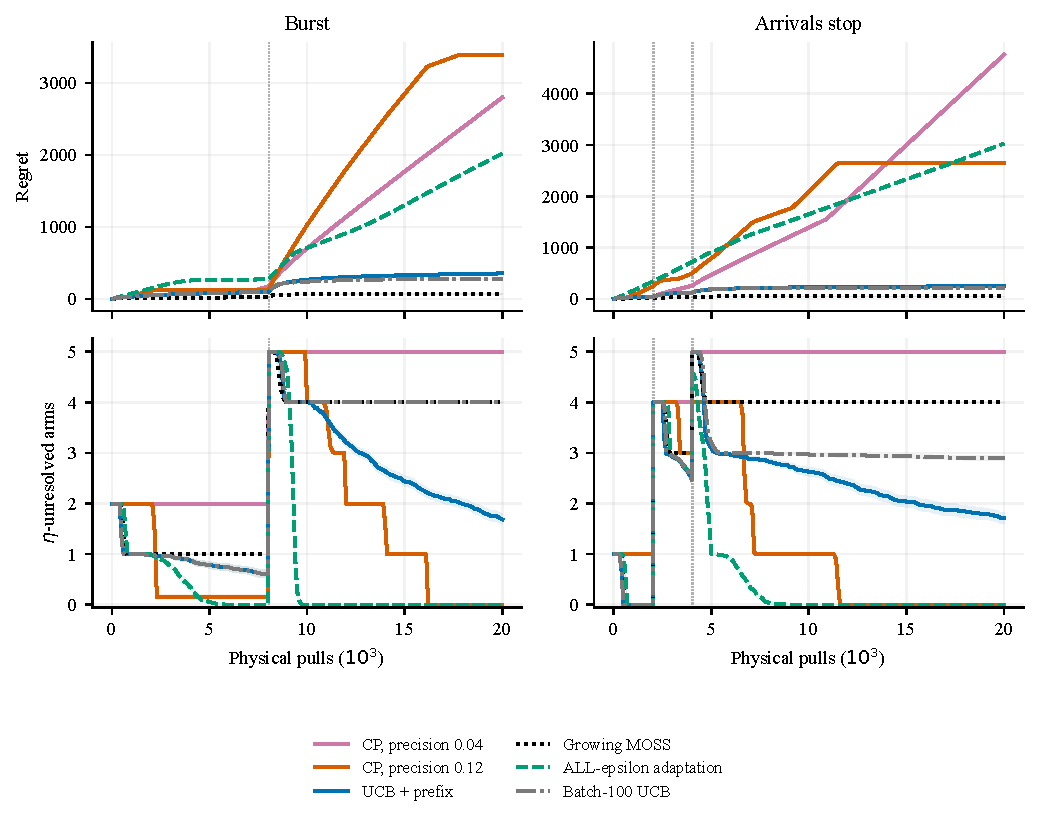
\includegraphics[width=.98\textwidth]{figures/fig_paths_pair2.pdf}
\caption{Additional paths for the burst and stopped-arrival environments.
The displayed policies, common potential reward streams, 160 replications,
and 1.96 Monte Carlo standard error bands are the same as in the main article.
Vertical lines mark actual arrivals. The full run-level data retain all nine
policies.}
\end{figure}

The compiled CP reference was compared to its original public class for
20,000 successive steps, checking choices, service flags, counts and reports.
The experiment records include per-run coverage and label errors, checkpoint
completion, service regret, and the three-part regret identity. Their largest
decomposition discrepancy was below $3.1\times10^{-12}$. These checks validate
the numerical implementation and accounting; they are not formal probability
certificates or proofs of the analytical lower bounds.

\section{Preserved figures from the original simulation study}
\label{app:original_simulations}
The original progressive step-up and near-tied top-set experiments are
preserved as an archived implementation record. Each scenario has 100
replications at $T=60{,}000$. The archived UCB-AA uses $M=5$ in the first
scenario and $M=4$ in the second, then commits to a fixed survivor pool.
The source snapshots and endpoint data show that later buffered arms are
not necessarily admitted. Its all-history empirical means and incumbent
reference comparisons also differ from the repaired prefix procedure.
The figures below therefore retain the original observations without
claiming validation of the revised fixed-budget algorithm.

\begin{figure}[p]
\centering
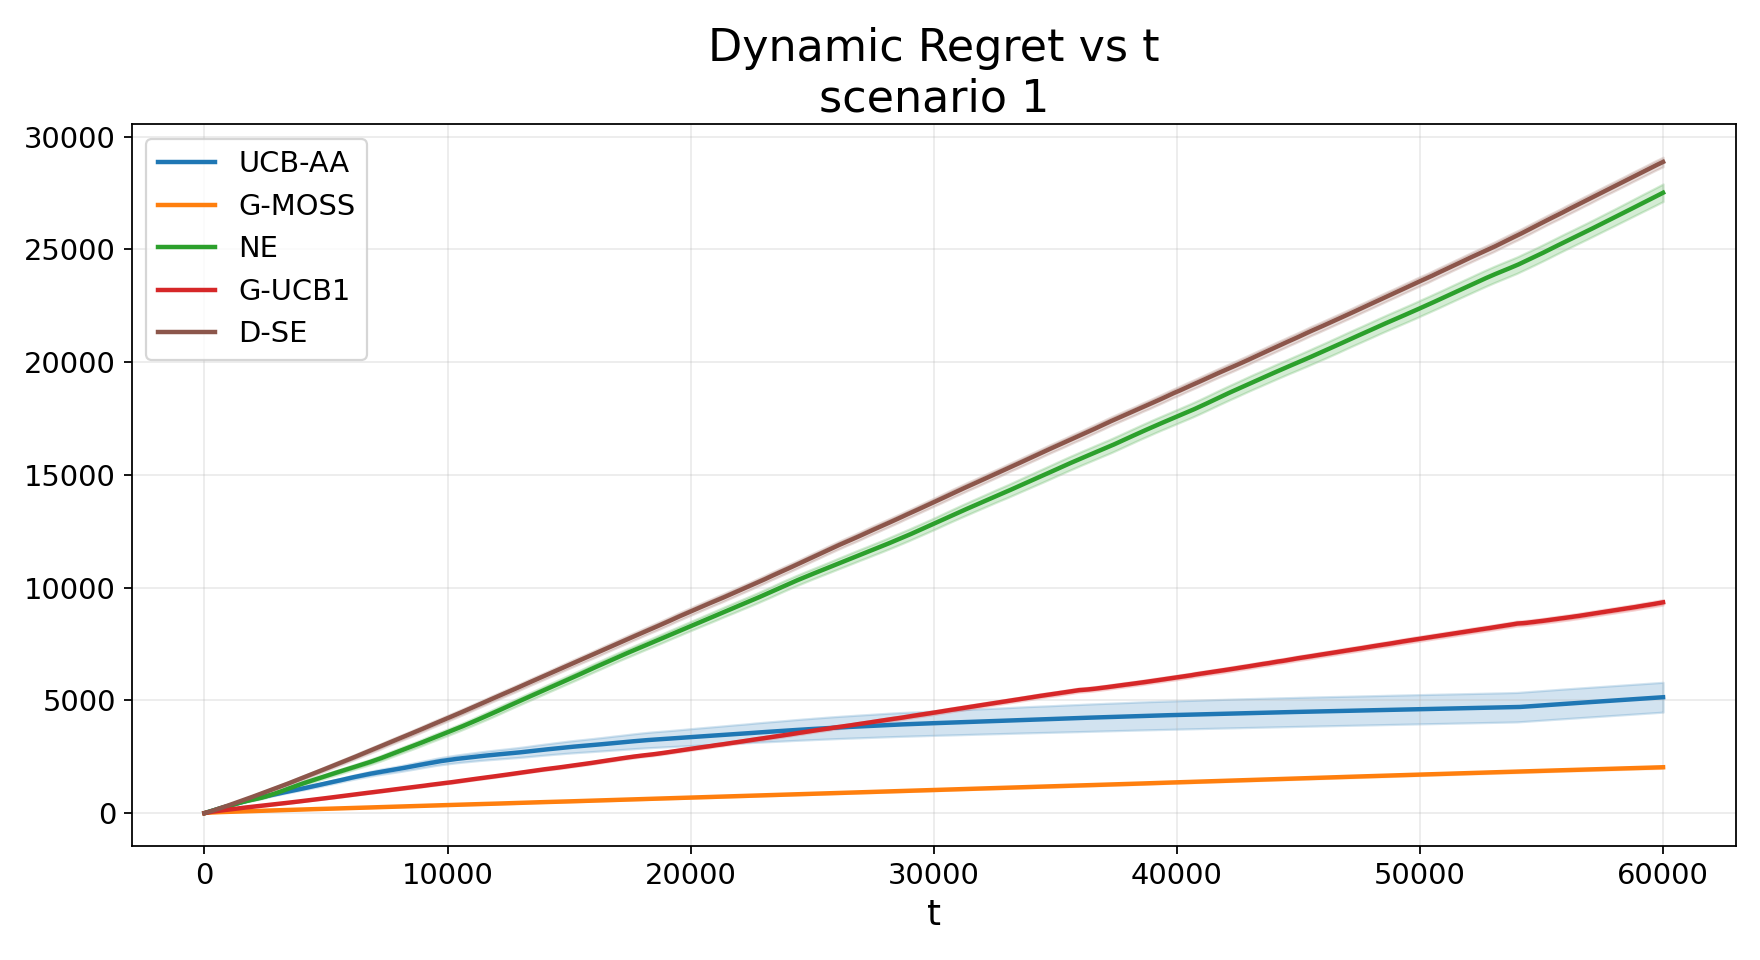
\includegraphics[width=.9\textwidth]{figures/original_submission/scenario_C_dynamic_regret_vs_t.png}
\par\medskip
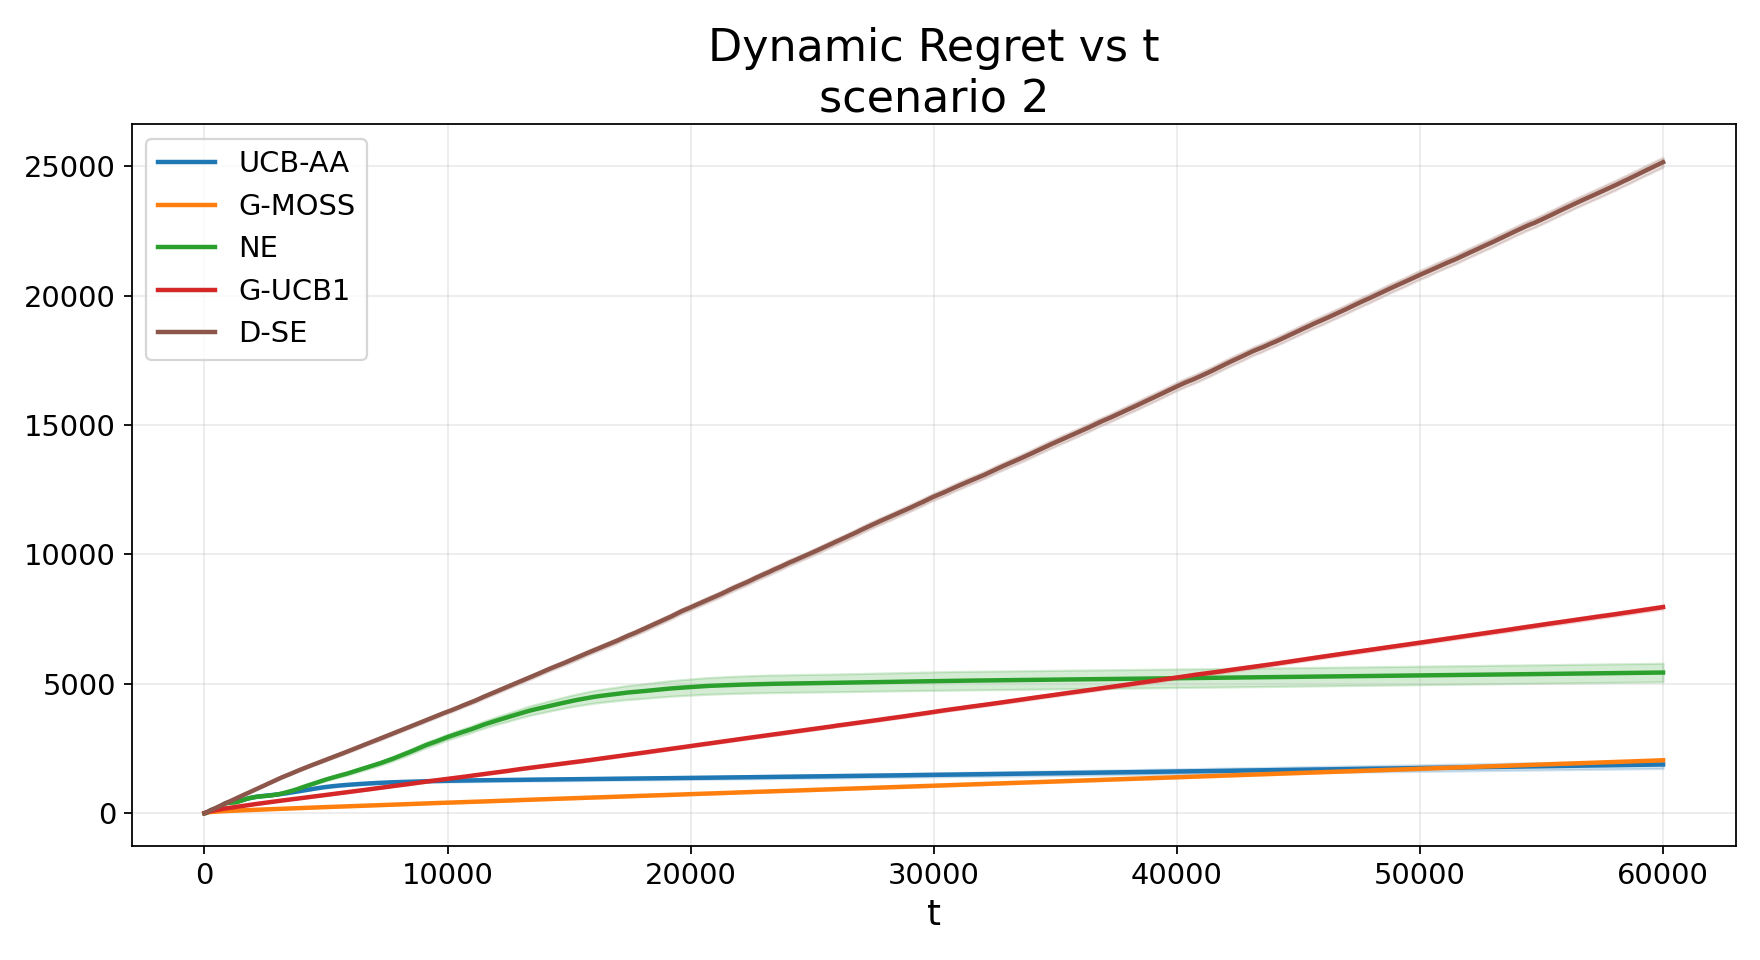
\includegraphics[width=.9\textwidth]{figures/original_submission/scenario_E_dynamic_regret_vs_t.png}
\caption{Preserved cumulative dynamic regret curves from the original
archived implementation. The step-up scenario is above and the near-tied
scenario below. The original uncertainty bands and 100 replications are
retained. The archived current-time MOSS index and finite-round UCB-AA
behavior are specified in the released source snapshots.}
\end{figure}

\begin{figure}[p]
\centering
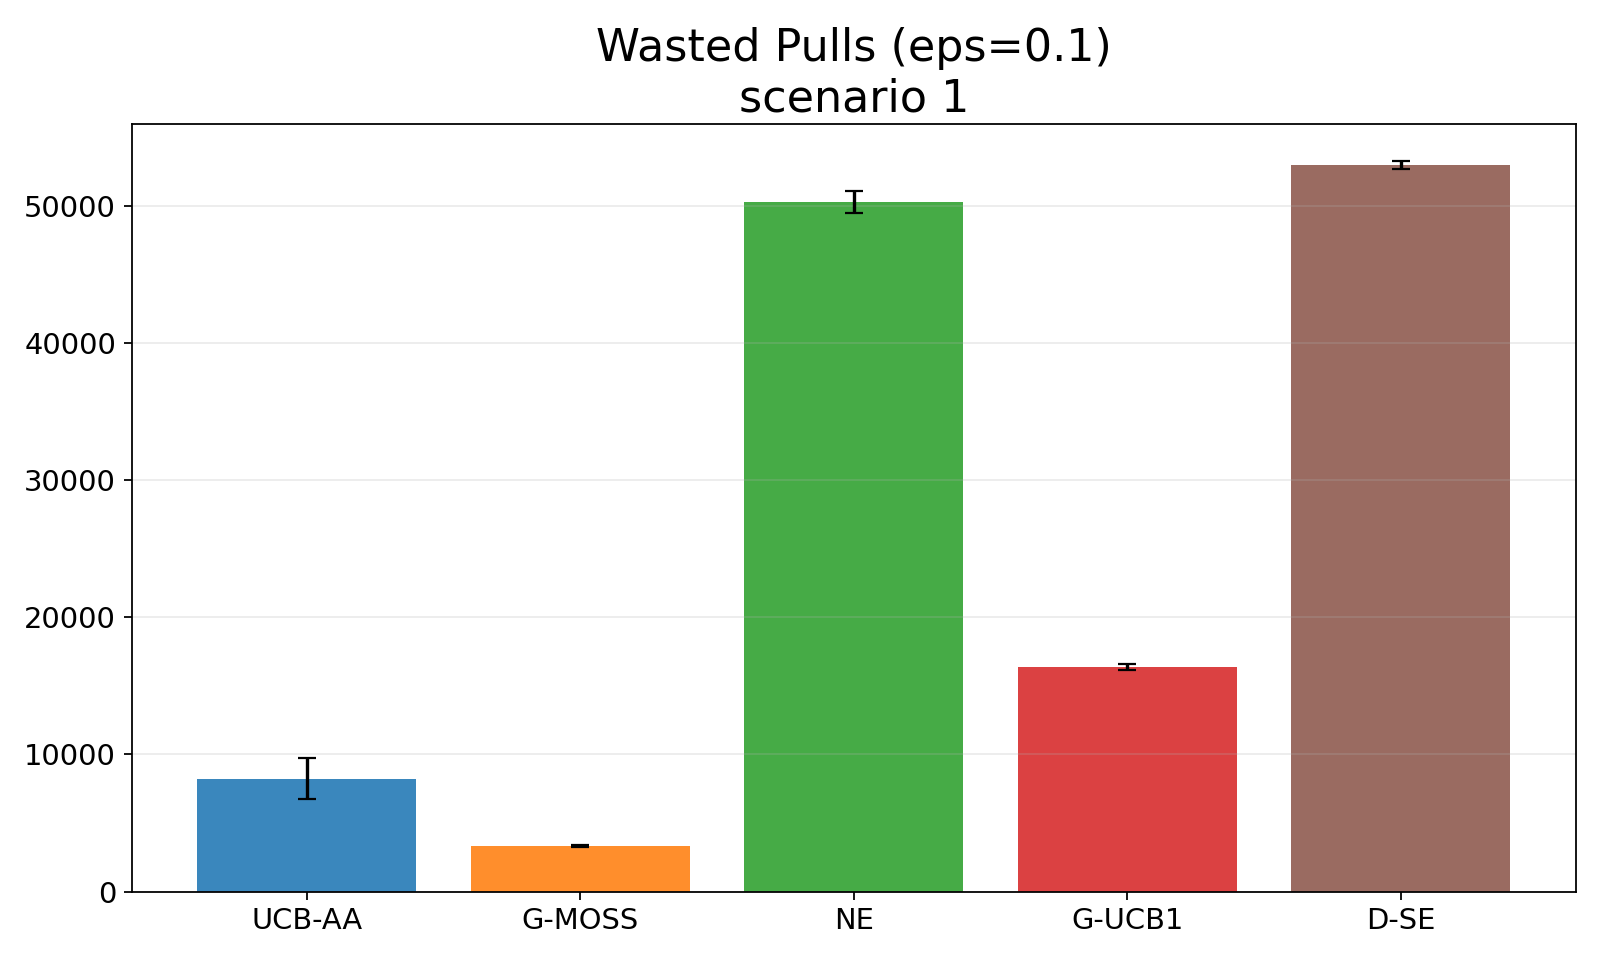
\includegraphics[width=.9\textwidth]{figures/original_submission/scenario_C_wasted_pulls_eps_0_1.png}
\par\medskip
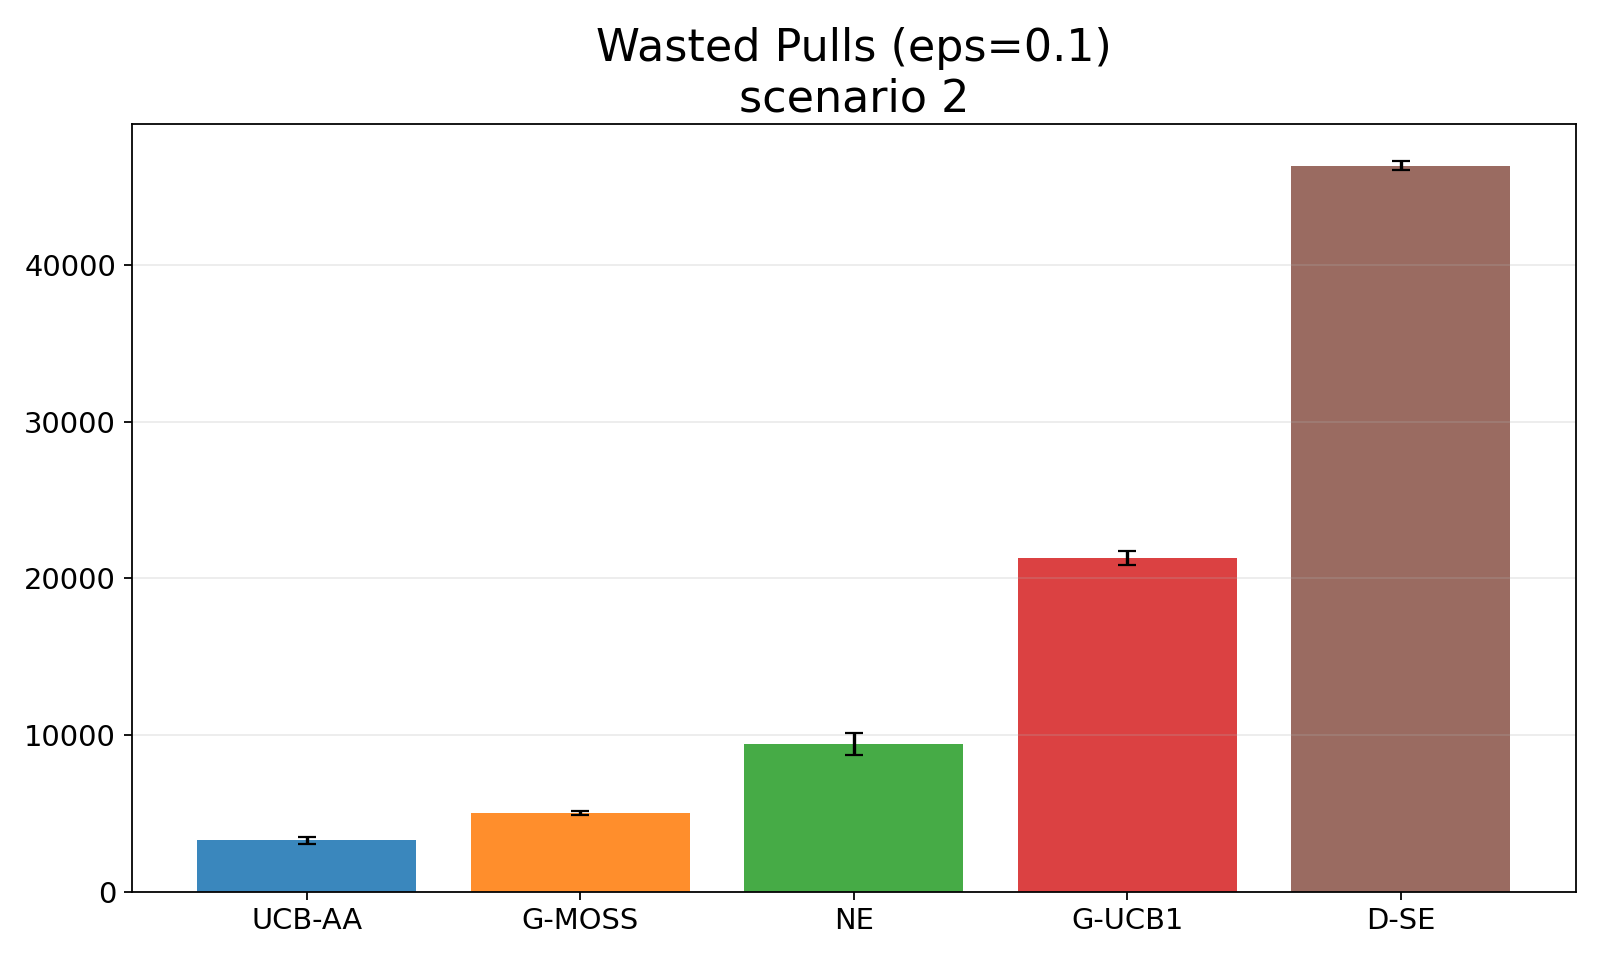
\includegraphics[width=.9\textwidth]{figures/original_submission/scenario_E_wasted_pulls_eps_0_1.png}
\caption{Preserved wasted-pull comparisons from the original step-up and
near-tied scenarios, with threshold $0.1$. These are archived implementation
results, not new simulations of the repaired algorithm.}
\end{figure}

\begin{figure}[p]
\centering
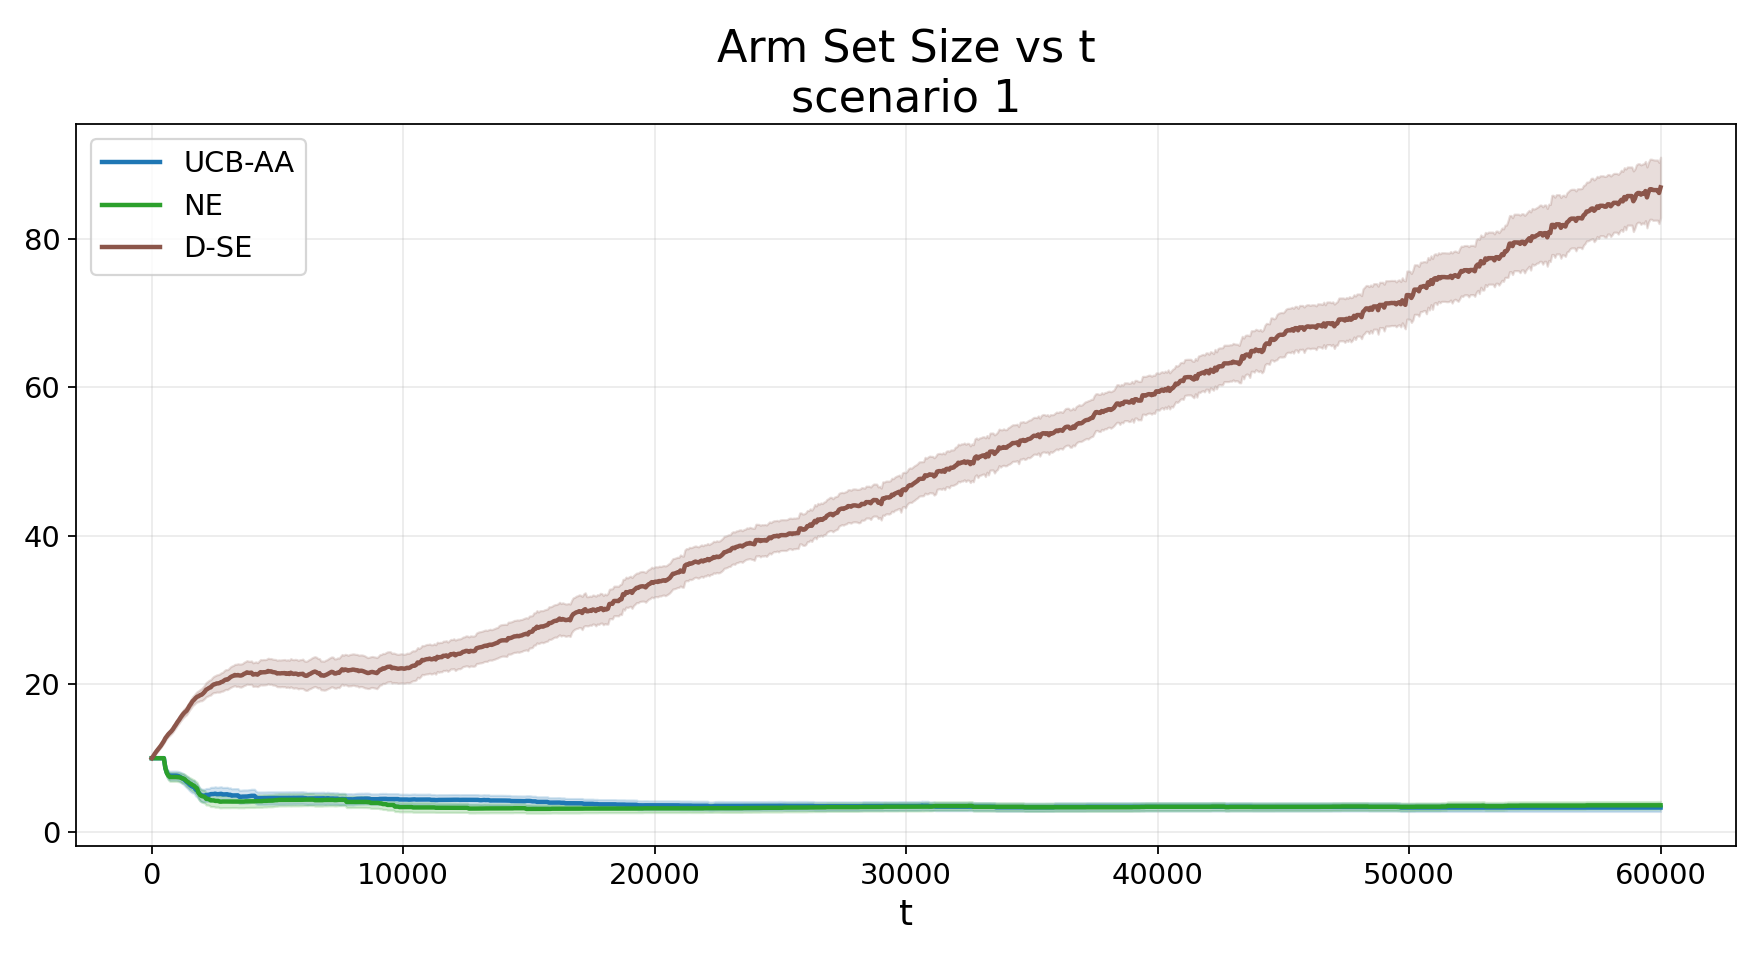
\includegraphics[width=.9\textwidth]{figures/original_submission/scenario_C_arm_set_size_vs_t.png}
\par\medskip
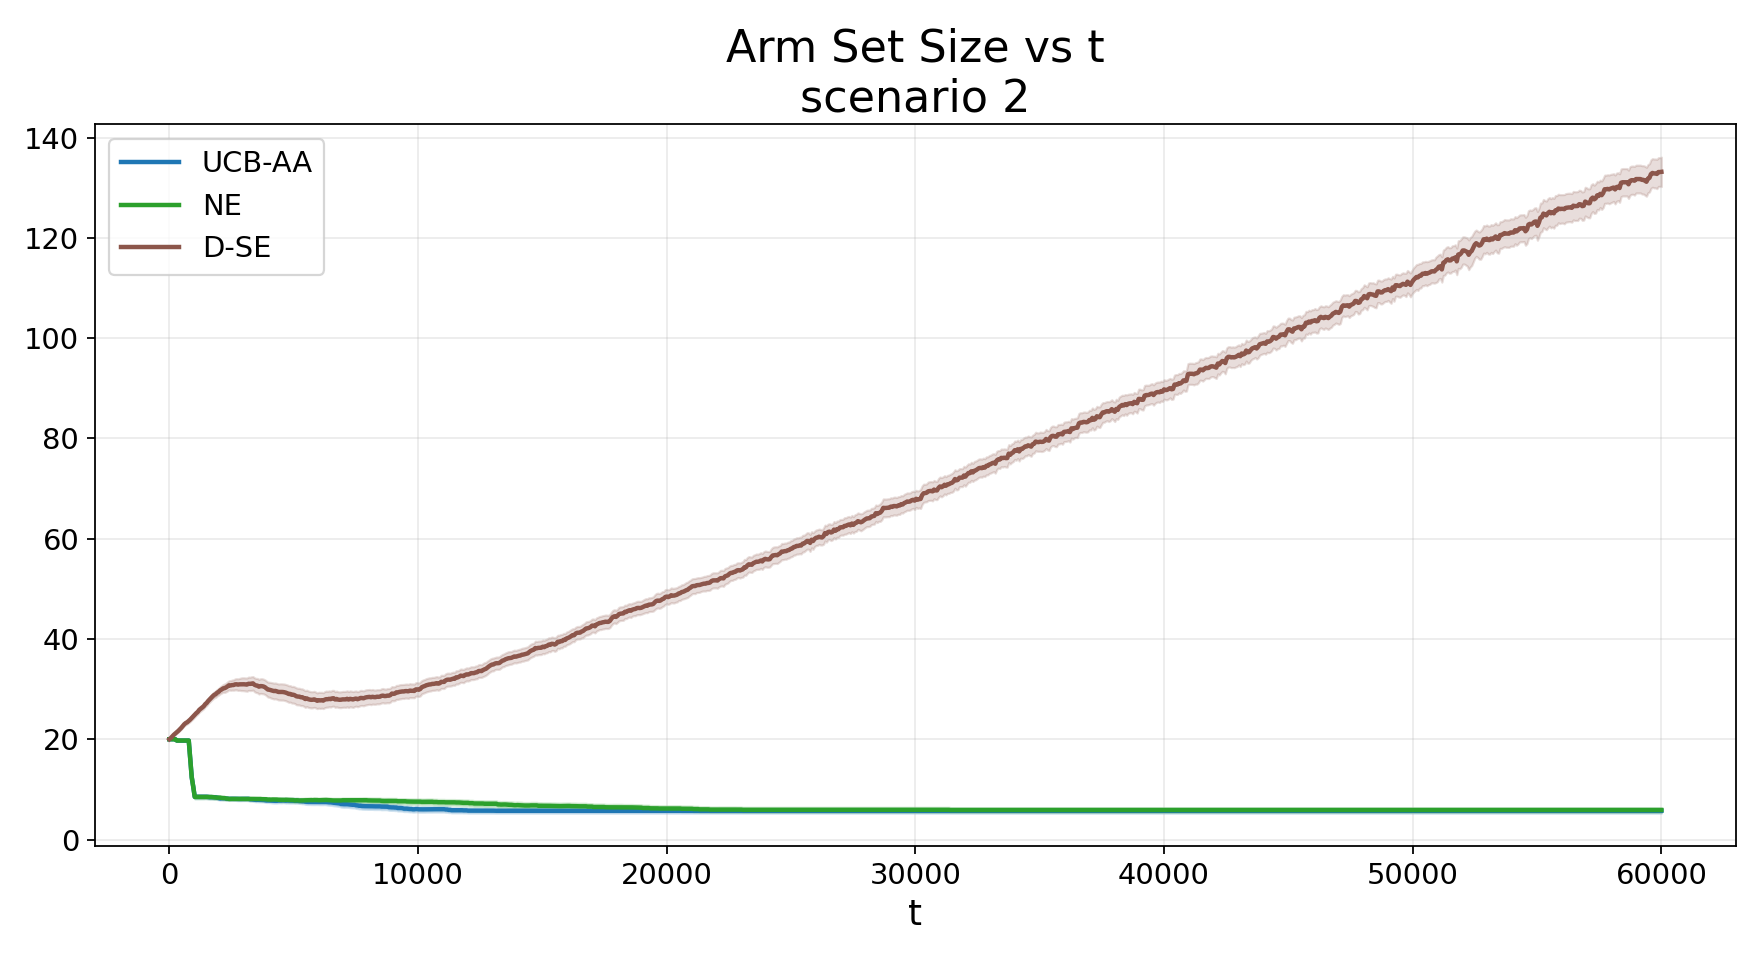
\includegraphics[width=.9\textwidth]{figures/original_submission/scenario_E_arm_set_size_vs_t.png}
\caption{Preserved original active-set curves. A smaller active set does
not imply that every later arrival was statistically excluded: the archived
UCB-AA implementation stops admission after its prescribed rounds.}
\end{figure}

\FloatBarrier
\bibliographystyle{plainnat}
\bibliography{references}
\end{document}
